%%%%%%%%%%%%%%%%%%%%%%%%%%%%%%%%%%%%%%%%%%%%%%%%%%%%%%%%%%%%%%%%%%%%%%%%%%%%%%%%
%% SANER 2027 Research Track submission.
%%
%% Format : IEEE Conference Proceedings, \documentclass[10pt,conference]{IEEEtran}
%%          (no "compsoc" / "compsocconf" option -- mandated by the CfP).
%% Limits : 10 pages of main text (all figures/tables/appendices included)
%%          + up to 2 extra pages containing ONLY references.
%% Review : double-blind. No author names/affiliations; own prior work cited
%%          in the third person; anonymous artifact links only.
%% Extra  : a Data Availability statement must directly follow the Conclusion.
%% Dates  : abstract 2026-09-21, paper 2026-09-25 (UTC-12), EasyChair.
%%
%% Build  : ./build.sh   (pdflatex -> bibtex -> pdflatex x2)
%% IEEEtran.cls / IEEEtran.bst are shipped next to this file so the paper
%% compiles on any TeX Live without texlive-publishers.
%%%%%%%%%%%%%%%%%%%%%%%%%%%%%%%%%%%%%%%%%%%%%%%%%%%%%%%%%%%%%%%%%%%%%%%%%%%%%%%%
\documentclass[10pt,conference]{IEEEtran}

%% --- Encoding / fonts ------------------------------------------------------
\usepackage[T1]{fontenc}
\usepackage[utf8]{inputenc}
\usepackage{microtype}

%% --- Core packages ---------------------------------------------------------
\usepackage{cite}              % IEEE-style compressed citation lists [1]-[3]
\usepackage{amsmath,amssymb}   % \operatorname*, \text, ...
\usepackage{graphicx}
\usepackage{booktabs}
\usepackage{xspace}
\usepackage{comment}           % \begin{comment} blocks used in the sections
\usepackage{xcolor}
\usepackage{balance}           % balance the two columns on the last page
\usepackage[most]{tcolorbox}   % RQ answer boxes + prompt box (loads tikz)
\usetikzlibrary{positioning,calc}

%% --- Links / cross-references (hyperref last, cleveref after hyperref) ----
\usepackage{url}
\usepackage[hidelinks]{hyperref}
\usepackage[capitalize,nameinlink]{cleveref}
% IEEE house style abbreviates "Figure" as "Fig." in running text.
\crefname{figure}{Fig.}{Figs.}
\Crefname{figure}{Fig.}{Figs.}
\crefname{table}{Table}{Tables}
\Crefname{table}{Table}{Tables}
\crefname{section}{Section}{Sections}
\Crefname{section}{Section}{Sections}
\crefname{equation}{Eq.}{Eqs.}
\Crefname{equation}{Eq.}{Eqs.}

%% --- RQ answer box ---------------------------------------------------------
\newtcolorbox{myboxi}[1][]{
  breakable,
  title=#1,
  colback=yellow!15,
  colbacktitle=white,
  coltitle=black,
  fonttitle=\bfseries,
  bottomrule=0pt,
  toprule=0pt,
  leftrule=3pt,
  rightrule=3pt,
  titlerule=0pt,
  arc=0pt,
  outer arc=0pt,
  colframe=black!60,
  left=4pt,
  right=4pt,
  top=3pt,
  bottom=3pt,
}

%% --- Prompt box (kept for compatibility; the prompt figure uses tikz) ------
\definecolor{mybkcolor}{HTML}{f2f2ff}
\newtcolorbox{promptbox}{
  colback=mybkcolor,
  colframe=black,
  boxrule=0.8pt,
  arc=4pt,
  left=4pt,
  right=4pt,
  top=4pt,
  bottom=4pt
}

%% --- Method names ----------------------------------------------------------
\newcommand{\votag}{VOTAG\xspace}
\newcommand{\ragtag}{RAGTAG\xspace}
\newcommand{\bragtag}{BRAGTAG\xspace}
\newcommand{\irc}{IRC\xspace}

%% --- Editing / reference helpers -------------------------------------------
\newcommand{\fixme}[1]{{\color{red}[#1]}}
\newcommand{\fixed}[1]{{\color{blue}#1}}
\newcommand{\change}[1]{{\color{green}#1}}
\newcommand{\rev}[1]{{\color{black}#1}}
\newcommand{\minor}[1]{{\color{red}#1}}
\newcommand{\secref}[1]{Section~\ref{sec:#1}}
\newcommand{\tabref}[1]{Table~\ref{tab:#1}}
\newcommand{\secsref}[2]{Sections~\ref{sec:#1}--\ref{sec:#2}}
\newcommand{\tabsref}[2]{Tables~\ref{tab:#1}--\ref{tab:#2}}
\newcommand{\figsref}[2]{Figs.~\ref{fig:#1}--\ref{fig:#2}}
\newcommand{\figref}[1]{Fig.~\ref{fig:#1}}
\newcommand{\eqaref}[1]{Eq.~\eqref{eq:#1}}
\newcommand{\lstref}[1]{Listing~\ref{lst:#1}}
\newcommand{\alref}[1]{Algorithm~\ref{al:#1}}

%% --- Run-in bold paragraph headings ----------------------------------------
\makeatletter
\newcommand{\myparagraph}[1]{%
  \@startsection{paragraph}{4}{\z@}%
    {0.4\baselineskip}%
    {-1em}%
    {\normalfont\normalsize\bfseries\raggedright}%
    *{#1}%
}
\newcommand{\myitparagraph}[1]{%
  \@startsection{paragraph}{4}{\z@}%
    {0.4\baselineskip}%
    {-1em}%
    {\normalfont\normalsize\bfseries\itshape\raggedright}%
    *{#1}%
}
\makeatother

% correct bad hyphenation here
\hyphenation{op-tical net-works semi-conduc-tor}

\begin{document}

\title{Can Retrieval-Augmented Few-Shot Prompting Match LoRA Fine-Tuning for Issue Report Classification? An Empirical Study}

%% Double-blind submission: anonymous author block.
\author{%
  \IEEEauthorblockN{Anonymous Author(s)}
  \IEEEauthorblockA{Anonymous Affiliation(s)}
}

%% Camera-ready author block (fill in after acceptance; keep commented for review).
\begin{comment}
\author{\IEEEauthorblockN{Author1}
\IEEEauthorblockA{Department of Computer Science\\
Bowling Green State University\\
Bowling Green, Ohio, USA\\
author1@bgsu.edu}
\and
\IEEEauthorblockN{Author2}
\IEEEauthorblockA{Department of Computer Science\\
Bowling Green State University\\
Bowling Green, Ohio, USA\\
author2@bgsu.edu}
\and
\IEEEauthorblockN{Author3}
\IEEEauthorblockA{Department of Computer Science\\
Bowling Green State University\\
Bowling Green, Ohio, USA\\
author3@bgsu.edu}
}
\end{comment}

\maketitle

%%%%%%%%%%%%%%%%%%%%%%%%%%%%%%%%%%%%%%%%%
%%          Sections
%%%%%%%%%%%%%%%%%%%%%%%%%%%%%%%%%%%%%%%%%
%%%%%%%%%%%%%%%%%%%%%%%%%%%%%%%%%%%%%%%%%
%%
%%          Section: Abstract
%%
%%%%%%%%%%%%%%%%%%%%%%%%%%%%%%%%%%%%%%%%%
% IEEE conference abstracts are a single unstructured paragraph. The ESEM
% structured version (Background / Aims / Method / Results / Conclusions) is
% preserved in the comment block at the bottom for reference.
\begin{abstract}
Classifying issue reports as bugs, feature requests, or questions helps developers triage them. Fine-tuned large language models (LLMs) give the best reported results, but fine-tuning needs a training run, reaches its best scores only with labeled issues pooled across projects, and must be repeated for new labels or a newer model. Retrieval-augmented few-shot prompting (RAG) instead shows the LLM the most similar labeled issues as examples and needs no training. To our knowledge, it has not been systematically evaluated for this task or compared with Low-Rank Adaptation (LoRA) fine-tuning. We conduct an empirical study with four Qwen2.5-Instruct models and 6{,}600 issue reports from eleven projects. \rag, like prior methods, most often labels questions as bugs, so a variant (\frag) removes bug-labeled examples when the retrieved issues suggest a question. Using only the target project's 300 labeled issues, \frag\ comes within 1.0 point of fine-tuning on all 3{,}300 labeled issues of the eleven projects in macro~$F_1$, a difference that is not statistically significant, and needs no training and 33\% less peak GPU memory on average. Without the filter, \rag\ trails fine-tuning by 2.8 points. Given the same labeled issues, both RAG variants outperform fine-tuning at every model size. RAG's inference is slower, and the two approaches make different errors: fine-tuning finds more bugs but over-predicts the bug label. With this filter, retrieval-augmented few-shot prompting preserves the macro~$F_1$ of LoRA fine-tuning with $11\times$ less labeled data per project, no training, and a third less GPU memory.
\end{abstract}

\begin{IEEEkeywords}
Issue classification, Retrieval-augmented generation, Fine-tuning, Large language models, Mining software repositories
\end{IEEEkeywords}

\begin{comment}
%% ESEM 2026 structured abstract (LIPIcs submission), kept for reference.
\myparagraph{Background.} Issue report classification (IRC) accelerates modern software maintenance, yet it remains a challenging task. State-of-the-art automated IRC methods fine-tune Large Language Models (LLMs) with Low-Rank Adaptation (LoRA), which is computationally expensive and must be repeated to incorporate newly labeled issue reports or whenever the model is swapped.

\myparagraph{Aims.} We empirically investigate the hypothesis that low-cost, retrieval-augmented generation (RAG)-based approaches can achieve competitive IRC performance with the LoRA fine-tuning baseline. If validated, this would introduce the possibility of cost-efficient IRC solutions; An avenue that, to our knowledge, remains unexplored in the literature.

\myparagraph{Method.} To test this hypothesis, we conduct a case study on the Qwen2.5-Instruct family, a set of open-source models with strong public-benchmark performance, evaluated at four parameter sizes to analyze the effect of model scale. We propose three retrieval-based methods, \knn, \rag, and \frag, each of which works by retrieving the top-$k$ most similar issues from an index of labeled issues and reasoning on them. Specifically, \knn\ assigns the label via a similarity-weighted vote over the retrieved neighbors; \rag\ presents the neighbors as classified examples in a few-shot LLM prompt; and \frag\ extends \rag\ with a more balanced retrieval scheme that better covers the label space. We evaluate all three methods against a LoRA fine-tuning baseline on an 11-project benchmark, under both \emph{project-specific} and \emph{project-agnostic} data scope settings.

\myparagraph{Results.} With project-specific data, \rag\ outperforms fine-tuning by 0.021--0.040 macro $F_1$ across all model sizes. Fine-tuning on cross-project data beats project-specific \rag\ by only 0.029 aggregate macro $F_1$ despite $11\times$ more labeled data. The balanced retrieval approach, \frag, closes this performance gap, achieving statistical equivalence with fine-tuning when using a retrieval fallback for invalid LLM outputs. Averaged across model sizes, retrieval-augmented few-shot prompting requires 33\% less peak GPU memory than fine-tuning.

\myparagraph{Conclusions.} Under our experimental setup and case study, RAG-based approaches demonstrate competitive performance against LoRA fine-tuning, suggesting they represent a viable and cost-efficient alternative for IRC, one that the literature has yet to fully explore.
\end{comment}

% !TEX root = ../SANER2027-main-labeling.tex
% Introduction
% Claims to support: headline claim + RQs + contributions
% SANER rewrite (2026-09-24): every paragraph is new text (blue). Numbers come from
% Section IV and paper/tables/{triangulation_all_cells,method_comparison_ci}.csv.

\section{Introduction}
\label{sec:01_intro}
Users and contributors of software projects report bugs, request features, and ask questions through issue trackers such as GitHub Issues~\cite{colavito2024leveraging}. Labeling each issue report with its type speeds up its resolution~\cite{liao2018exploring} and supports issue prioritization~\cite{catolino2019not}, issue assignment~\cite{wu2022spatial}, and developer onboarding~\cite{santos2023tag, aracena2025applying}. Yet labels are rarely used~\cite{kallis2019ticket} and often wrong~\cite{antoniol2008bug, herzig2013s}, and manually assigning them is laborious~\cite{fan2017road}. To address these problems, many studies propose methods for automated issue report classification (\irc) and typically evaluate them on the labels \emph{bug}, \emph{feature}, and \emph{question}~\cite{kallis2019ticket, izadi2022catiss, kallis2024nlbse, colavito2025benchmarking, heo2025study}.

Most \irc\ methods learn from labeled issues. Early work trained classic machine-learning classifiers~\cite{antoniol2008bug, kallis2019ticket, pandey2017automated}, later work fine-tuned pre-trained transformer models~\cite{izadi2022catiss, trautsch2022predicting, colavito2022issue, wang2021well}, and recent work applies large language models (LLMs)~\cite{colavito2025benchmarking, aracena2025applying, heo2025study}. Among LLM-based methods, fine-tuning on labeled issues gives the best reported results~\cite{heo2025study, aracena2025applying, aracena2024applyinglargelanguagemodels}, with Low-Rank Adaptation (LoRA~\cite{hu2022lora}) for open models. Fine-tuning, however, adds a training run that must be repeated to learn from newly labeled issues or to adopt a newer model~\cite{fan2017road, kallis2019ticket}.

LLMs can also use labeled issues without training. Through in-context learning, a model infers a task from a few labeled examples in its prompt~\cite{brown2020language}, and choosing the labeled examples most similar to the query issue can outperform choosing them at random~\cite{liu2022makes, yu2023retrieval}. With such retrieval-augmented few-shot prompting (\rag), a newly labeled issue only needs to be indexed, and the LLM can be replaced without retraining. For future work, Heo and Lee~\cite{heo2025study} suggest few-shot prompting, and Aracena et~al.~\cite{aracena2025applying} suggest retrieval augmentation to reduce the need for extensive fine-tuning and to help with ambiguous labels such as question. To our knowledge, however, retrieval-augmented few-shot prompting has not been systematically evaluated for \irc\ or compared with LoRA fine-tuning.

This paper does both. In an empirical study, we use four Qwen2.5-Instruct models of 3B to 32B parameters~\cite{yang2024qwen25} and Heo and Lee's balanced benchmark of issue reports from eleven projects~\cite{heo2025study}, each with 300 labeled and 300 test issues. Following Heo and Lee, the retrieval index and the fine-tuning data come either from the target project's 300 labeled issues alone (the project-specific setting) or from all 3{,}300 labeled issues of the eleven projects (the project-agnostic setting).

The retrieved examples are the labeled issues most similar to the query, so we first test how well their labels alone predict the query's label. We label the query by a similarity-weighted vote over these neighbors, without an LLM (\knn). Using only the target project's labeled issues, the vote reaches 59.5\% macro~$F_1$, so the neighbors carry label information that an LLM could use. \rag therefore shows these neighbors to the LLM as examples. As with prior \irc\ methods~\cite{colavito2024impact, colavito2025benchmarking}, \rag's most frequent error is labeling questions as bugs, and we target this error by removing the bug-labeled examples for suspected questions (\frag).

In this study, we answer four research questions.

\myparagraph{RQ1} \emph{How effectively can retrieval alone classify issue reports, and at what point does adding more retrieved neighbors stop helping?} The \knn baseline peaks at 59.5\% macro $F_1$ with 15 neighbors from the target project and at 60.4\% with 16 neighbors from all eleven projects. It is weakest on questions and labels 32\% of them as bugs.

\myparagraph{RQ2} \emph{How well does retrieval-augmented few-shot prompting classify issue reports, and how does performance vary with the number of in-context examples?} \rag\ shows the LLM $k$ examples, for seven values of $k$ from 0 (zero-shot prompting) up to 15, the bound set by \knn's peaks. Every configuration with at least one example outperforms both zero-shot prompting and \knn's best result. At each model's best $k$, \rag\ reaches 69.7--76.7\% macro $F_1$ with the target project's labeled issues. Retrieved examples lower the share of questions predicted as bugs from 46--59\% at zero-shot to 26--36\% at the best $k$, but question remains the weakest class.

\myparagraph{RQ3} \emph{Can a balanced retrieval intervention reduce question-to-bug misclassification and improve retrieval-augmented few-shot performance?} The models label many questions as bugs even without examples, so we hypothesize that bug-labeled neighbors retrieved for a question reinforce this error. \Frag\ therefore removes the bug-labeled examples from the prompt, unless they outnumber the question-labeled ones by more than a small margin. It scores higher than \rag\ at every $k{\ge}6$ for all four models, and by 1.5--2.4 points at each method's best $k$ (95\% confidence intervals exclude zero). It also lowers the share of questions predicted as bugs to 19--27\%, at the cost of bug recall.

\myparagraph{RQ4} \emph{How do the two RAG variants compare with LoRA fine-tuning in classification performance, peak GPU memory, and labeled-data needs?} With the same 300 labeled issues of the target project, \rag\ and \frag\ at their best $k$ score higher than LoRA fine-tuning at every model size, by 2.1--6.0 points in macro~$F_1$. When fine-tuning instead uses all 3{,}300 labeled issues of the eleven projects, \rag\ trails it by 2.8 points on average over the four model sizes, and \frag\ trails it by 1.0 point, a difference that is not statistically significant. Once a \knn\ fallback replaces invalid LLM outputs, \frag\ matches fine-tuning (0.1 point ahead on average). Beyond macro~$F_1$, fine-tuning finds more of the actual bugs but over-predicts the bug label, whereas \frag\ makes fewer false bug predictions at most model sizes. The question-to-bug confusion persists under every method we test, including fine-tuning. Both RAG variants need no training, 300 instead of 3{,}300 labeled issues, and 33\% less peak GPU memory than fine-tuning on average.

Overall, retrieval-augmented few-shot prompting is competitive with LoRA fine-tuning while requiring no training, and the two approaches trade different strengths. Which one suits a project depends on its labeled data, its GPU budget, and whether a missed bug or a false bug label costs it more. Our main contributions are the following:

\begin{itemize}
  \item A similarity-weighted $k$-nearest-neighbor baseline (\knn) that measures how much label information the retrieved neighbors carry, bounds the number of in-context examples, and serves as a fallback for invalid LLM outputs.

  \item An evaluation of retrieval-augmented few-shot prompting (\rag) for \irc\ across four model sizes and seven values of $k$.

  \item A training-free retrieval intervention (\frag) that reduces the question-to-bug misclassification known from prior \irc\ work, at the cost of bug recall.

  \item A comparison of \rag and \frag with LoRA fine-tuning of the same models on the same labeled issues, in classification performance, peak GPU memory, and labeled-data needs, reported with paired bootstrap confidence intervals and per-class precision and recall.
\end{itemize}

The rest of the paper is organized as follows. \Cref{sec:03_approach} describes our methods and the fine-tuning baseline, \Cref{sec:setup} the experimental setup, and \Cref{sec:evaluations} the results. \Cref{sec:discussion} analyzes failure cases and practical implications, \Cref{sec:02_related} reviews related work, \Cref{sec:threats} discusses threats to validity, and \Cref{sec:conclusion} concludes and outlines future work.

% !TEX root = ../SANER2027-main-labeling.tex
% Related Work: each paragraph describes a line of prior work, then contrasts it with this study.
% Facts about the cited papers (quotes, pages): docs/reframe/RW_DOSSIER.md

\section{Related Work}
\label{sec:02_related}

\myparagraph{Supervised Issue Report Classification} Early \irc\ studies trained classic machine-learning classifiers on issue text~\cite{antoniol2008bug, kallis2019ticket, fan2017road}. Later work fine-tuned transformer encoders~\cite{colavito2022issue, bharadwaj2022github, trautsch2022predicting, izadi2022catiss, izadi2022predicting}. For instance, Izadi et al.~\cite{izadi2022catiss} and Trautsch et al.~\cite{trautsch2022predicting} fine-tuned RoBERTa~\cite{liu2019roberta} and seBERT~\cite{von2022validity}, respectively, to classify issues as bugs, features, or questions, and Siddiq and Santos trained a BERT classifier on more than 800{,}000 labeled issues~\cite{siddiq2022bert}. Colavito et al. fine-tuned a sentence encoder with SetFit on about 200 labeled issues~\cite{colavito2023few, colavito2024large}. All of these methods train a dedicated classifier on the labeled issues. This study instead holds the LLM fixed and varies only how the labeled issues are used, as examples in the prompt or as training data for LoRA, so its baseline is LoRA fine-tuning of the same models rather than a different classifier. Our sentence encoder is not trained and serves only to retrieve the neighbors.

\myparagraph{LLMs for Issue Report Classification} LLMs can classify issues without task-specific training~\cite{heo2025study, colavito2024leveraging, colavito2025benchmarking}, although their zero-shot performance varies across datasets~\cite{colavito2025benchmarking}. Colavito et al.~\cite{colavito2025benchmarking, colavito2024leveraging} added one or two randomly chosen labeled examples per class to the prompt, and in their benchmark these examples did not improve over zero-shot prompting for most models~\cite{colavito2025benchmarking}. The best reported results come from GPT models fine-tuned on labeled issues through OpenAI's API~\cite{aracena2024applyinglargelanguagemodels, aracena2025applying, heo2025study}. Open models such as Llama-3.1-8B and DeepSeek-R1-Distill-Llama-8B were fine-tuned with LoRA~\cite{hu2022lora} and scored lower~\cite{heo2025study, aracena2025applying}. Heo and Lee trained each classifier either on one project's issues or on the issues pooled from eleven projects~\cite{heo2025study}. We adopt their benchmark and both settings. These studies report cost as training time, inference time, or API prices~\cite{heo2025study, aracena2025applying, colavito2025benchmarking}, not as GPU memory. For future work, Heo and Lee suggest few-shot prompting, and Aracena et al. suggest retrieving relevant past issues to reduce the need for extensive fine-tuning~\cite{heo2025study, aracena2025applying}. This study evaluates both suggestions together. We show the LLM the labeled issues most similar to the query, up to 15 of them, and compare this with LoRA fine-tuning of the same four open models on the same labeled issues, in both of Heo and Lee's settings, including peak GPU memory. \rag\ outperforms zero-shot prompting at every model size and every $k$ (\Cref{sec:rq1}). To our knowledge, retrieval-augmented few-shot prompting has not been systematically evaluated for \irc\ or compared with LoRA fine-tuning before.

\myparagraph{Retrieved In-Context Examples} In-context learning lets an LLM infer a task from labeled examples in its prompt~\cite{brown2020language}. Choosing the examples most similar to the query outperforms random choice for GPT-3 on NLP benchmarks~\cite{liu2022makes}, and Milios et al. retrieve examples with a frozen sentence encoder to classify intents and emotions with up to 150 labels~\cite{milios2023context}. Yu et al., by contrast, train both the retriever and a RoBERTa classifier~\cite{yu2023retrieval}. In software engineering, LLM-Cure assigns app reviews to features with five fixed examples in its prompt~\cite{assi2026llm}. Closest to our work, Dinç and Tüzün show LLMs the five most similar labeled reports, retrieved with the same sentence encoder and FAISS library as ours, to decide whether Firefox bug reports are valid. In their study, fine-tuned encoders score higher than the prompted LLMs, and the authors name a sweep over $k$ and filtering the neighbors as future work~\cite{dincc2025judge}. For masked language models of under one billion parameters, Logan et al. found fine-tuning more accurate than in-context learning and more robust to the prompt wording~\cite{logan2021cuttingpromptsparameterssimple}. This study brings retrieved examples to three-label \irc\ across eleven projects. It sweeps $k$ up to where a vote over the neighbors' labels peaks, separates what retrieval and the LLM contribute with the \knn\ and zero-shot references (\Cref{sec:rq1}), and compares with LoRA fine-tuning of the same 3B to 32B instruction-tuned LLMs. In our study, \rag\ trails fine-tuning on the pooled issues by 2.8 points; with the example filter, the gap shrinks to 1.0 point and is not statistically significant (\Cref{sec:rq3}).

\myparagraph{Label Bias in the Examples} Ma et al. observe that similarity-based selection tends to pick examples whose labels match the query's, and that LLMs then lean toward the labels that dominate the context~\cite{ma2023fairnessguidedfewshotpromptinglarge}. Milios et al. report that the neighbors retrieved for the neutral emotion rarely carry that label, and suspect that retrieval limits performance on it~\cite{milios2023context}. We see a similar pattern for questions. On our validation split, true questions retrieve nearly as many bug-labeled as question-labeled neighbors (\Cref{sec:approach-bragtag}), and the models label many questions as bugs even without examples (\Cref{sec:rq1}). We hypothesize that the bug-labeled examples reinforce this error. Ma et al. reduce the bias by searching, with extra LLM calls, for one low-bias set of examples, scored by the entropy of the LLM's label distribution on a content-free input~\cite{ma2023fairnessguidedfewshotpromptinglarge}. Dinç and Tüzün add a judge LLM that sees the votes of several classifiers~\cite{dincc2025judge}. \Frag\ instead keeps per-query retrieval and applies a count rule to the neighbors' labels, removing the bug-labeled examples for suspected questions without an extra LLM call or access to output probabilities. It raises macro~$F_1$ over \rag\ by 1.5--2.4 points at the cost of bug recall (\Cref{sec:rq2}).

% Prior-work context for the question-to-bug confusion (ESEM reviewer C).
% Evidence, quotes and page numbers: docs/research/QUESTION_BUG_PRIOR_WORK.md
\myparagraph{Question-to-Bug Misclassification} In \irc\ studies that include both bug and question labels, question is often the hardest class to identify, and misclassified questions are most often labeled as bugs. For example, almost all methods in the NLBSE'24 tool competition struggled with question~\cite{kallis2024nlbse}, and on the same dataset, the two best-performing zero-shot LLMs labeled 46--54\% of questions as bugs~\cite{colavito2025benchmarking}. Fine-tuned LLMs also score lowest on question in aggregate~\cite{aracena2025applying, heo2025study}. Our results show the same pattern: every method we evaluate, fine-tuning included, labels many questions as bugs (\Cref{sec:rq1,sec:rq3}). As remedies, Aracena et al.~\cite{aracena2025applying} suggest retrieval augmentation, particularly for ambiguous labels such as question, and a first classification stage that separates questions from bug and feature reports. In our study, retrieved examples lower the share of questions labeled as bugs from 46--59\% under zero-shot prompting to 26--36\%, and \frag\ lowers it further to 19--27\% without an extra classification stage, but neither removes the confusion.

Prior work offers several explanations for this confusion. Question is often the smallest class in the training data~\cite{izadi2022catiss, bharadwaj2022github}, but our benchmark is balanced and the confusion remains, so imbalance alone does not explain it. Some questions read like bug reports because they describe unexpected behavior, contain error messages~\cite{colavito2024impact}, or lack explicit interrogative markers~\cite{aracena2025applying}. Our failure analysis (\Cref{sec:disc-failures}) finds a related cause: questions filed under a bug-report template lead the model to predict bug regardless of their content. Finally, a label can depend on information outside the report, such as a maintainer's later diagnosis~\cite{colavito2024impact}. Likewise, the label-noise cases in our failure analysis have labels that do not match their content and cannot be inferred from the report text.

% !TEX root = ../SANER2027-main-labeling.tex
% Approach
% kNN voting baseline, RAG, filtered RAG (with its calibration), LoRA fine-tuning baseline

\section{Approach}
\label{sec:03_approach}

\begin{comment}
\begin{figure}[t]
    \centering
    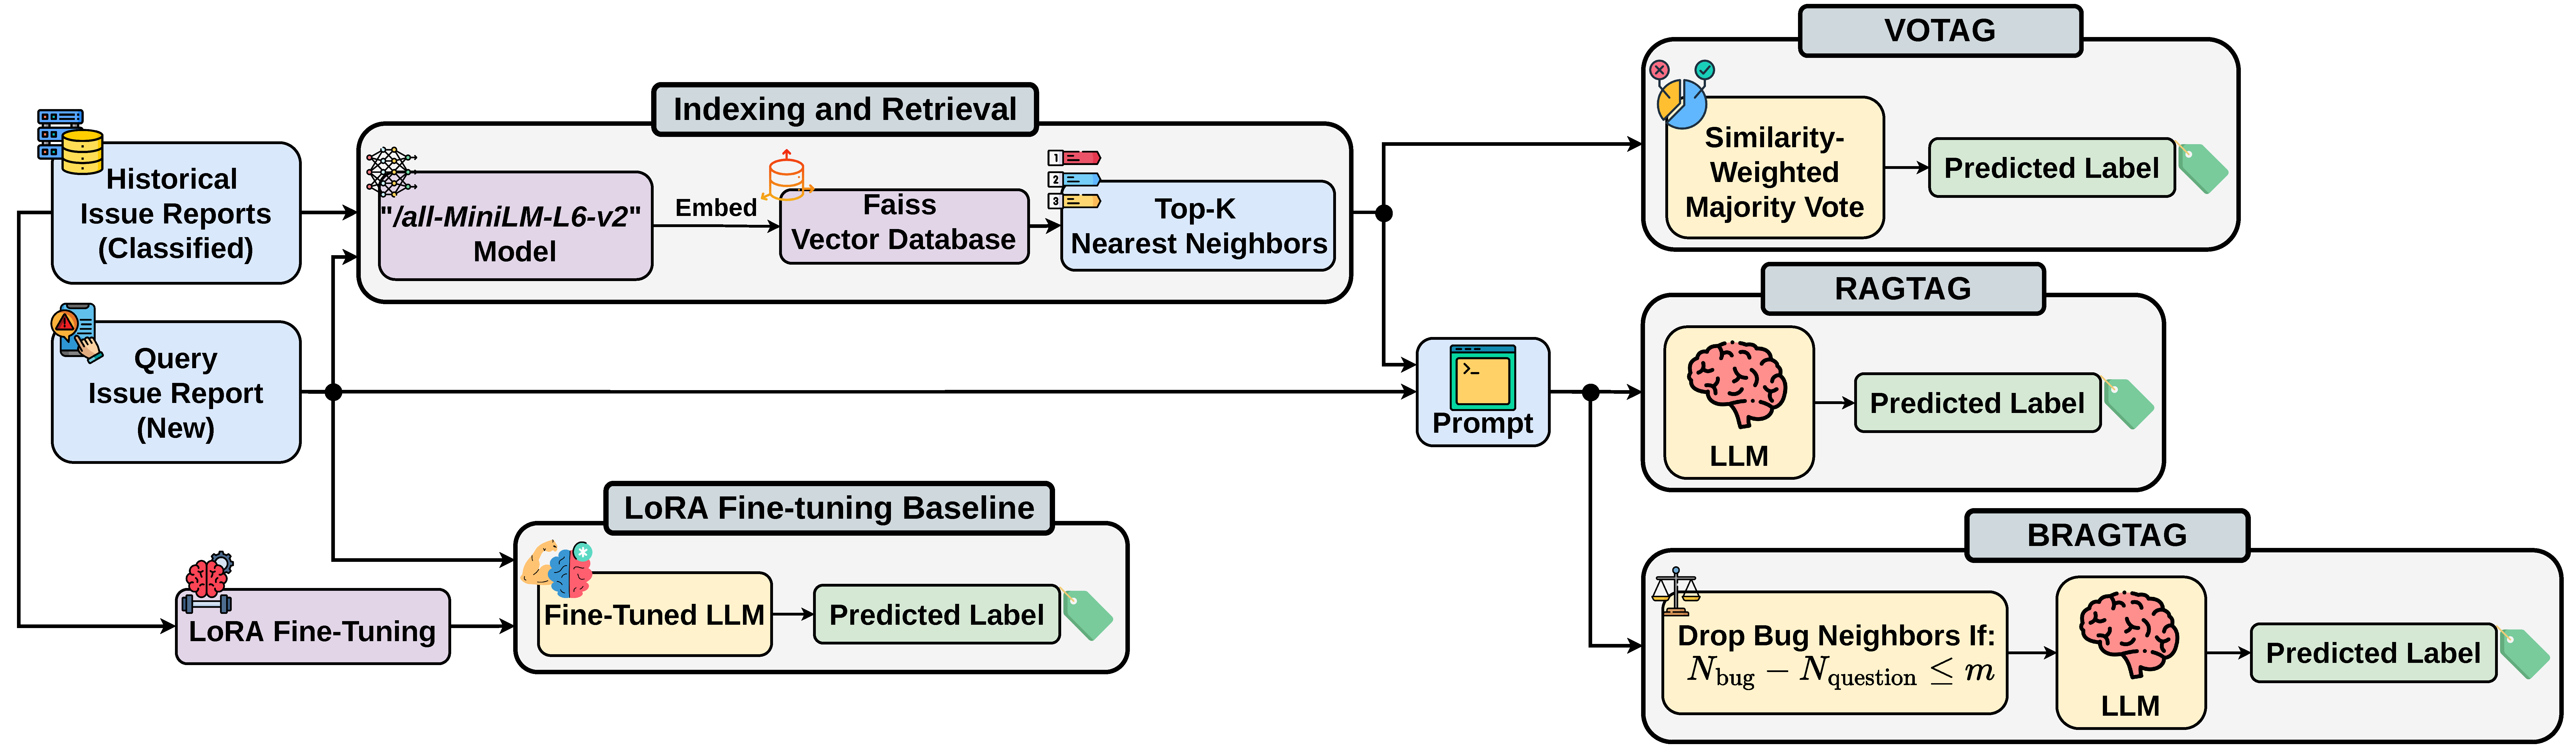
\includegraphics[width=\linewidth]{figures/app_ov.pdf}
    \caption{Overview of the $k$NN voting baseline, retrieval-augmented few-shot prompting (RAG), filtered RAG, and the LoRA fine-tuning baseline.}
    \label{fig:approach-overview}
\end{figure}
\end{comment}

\begin{figure*}[!t]
    \centering
    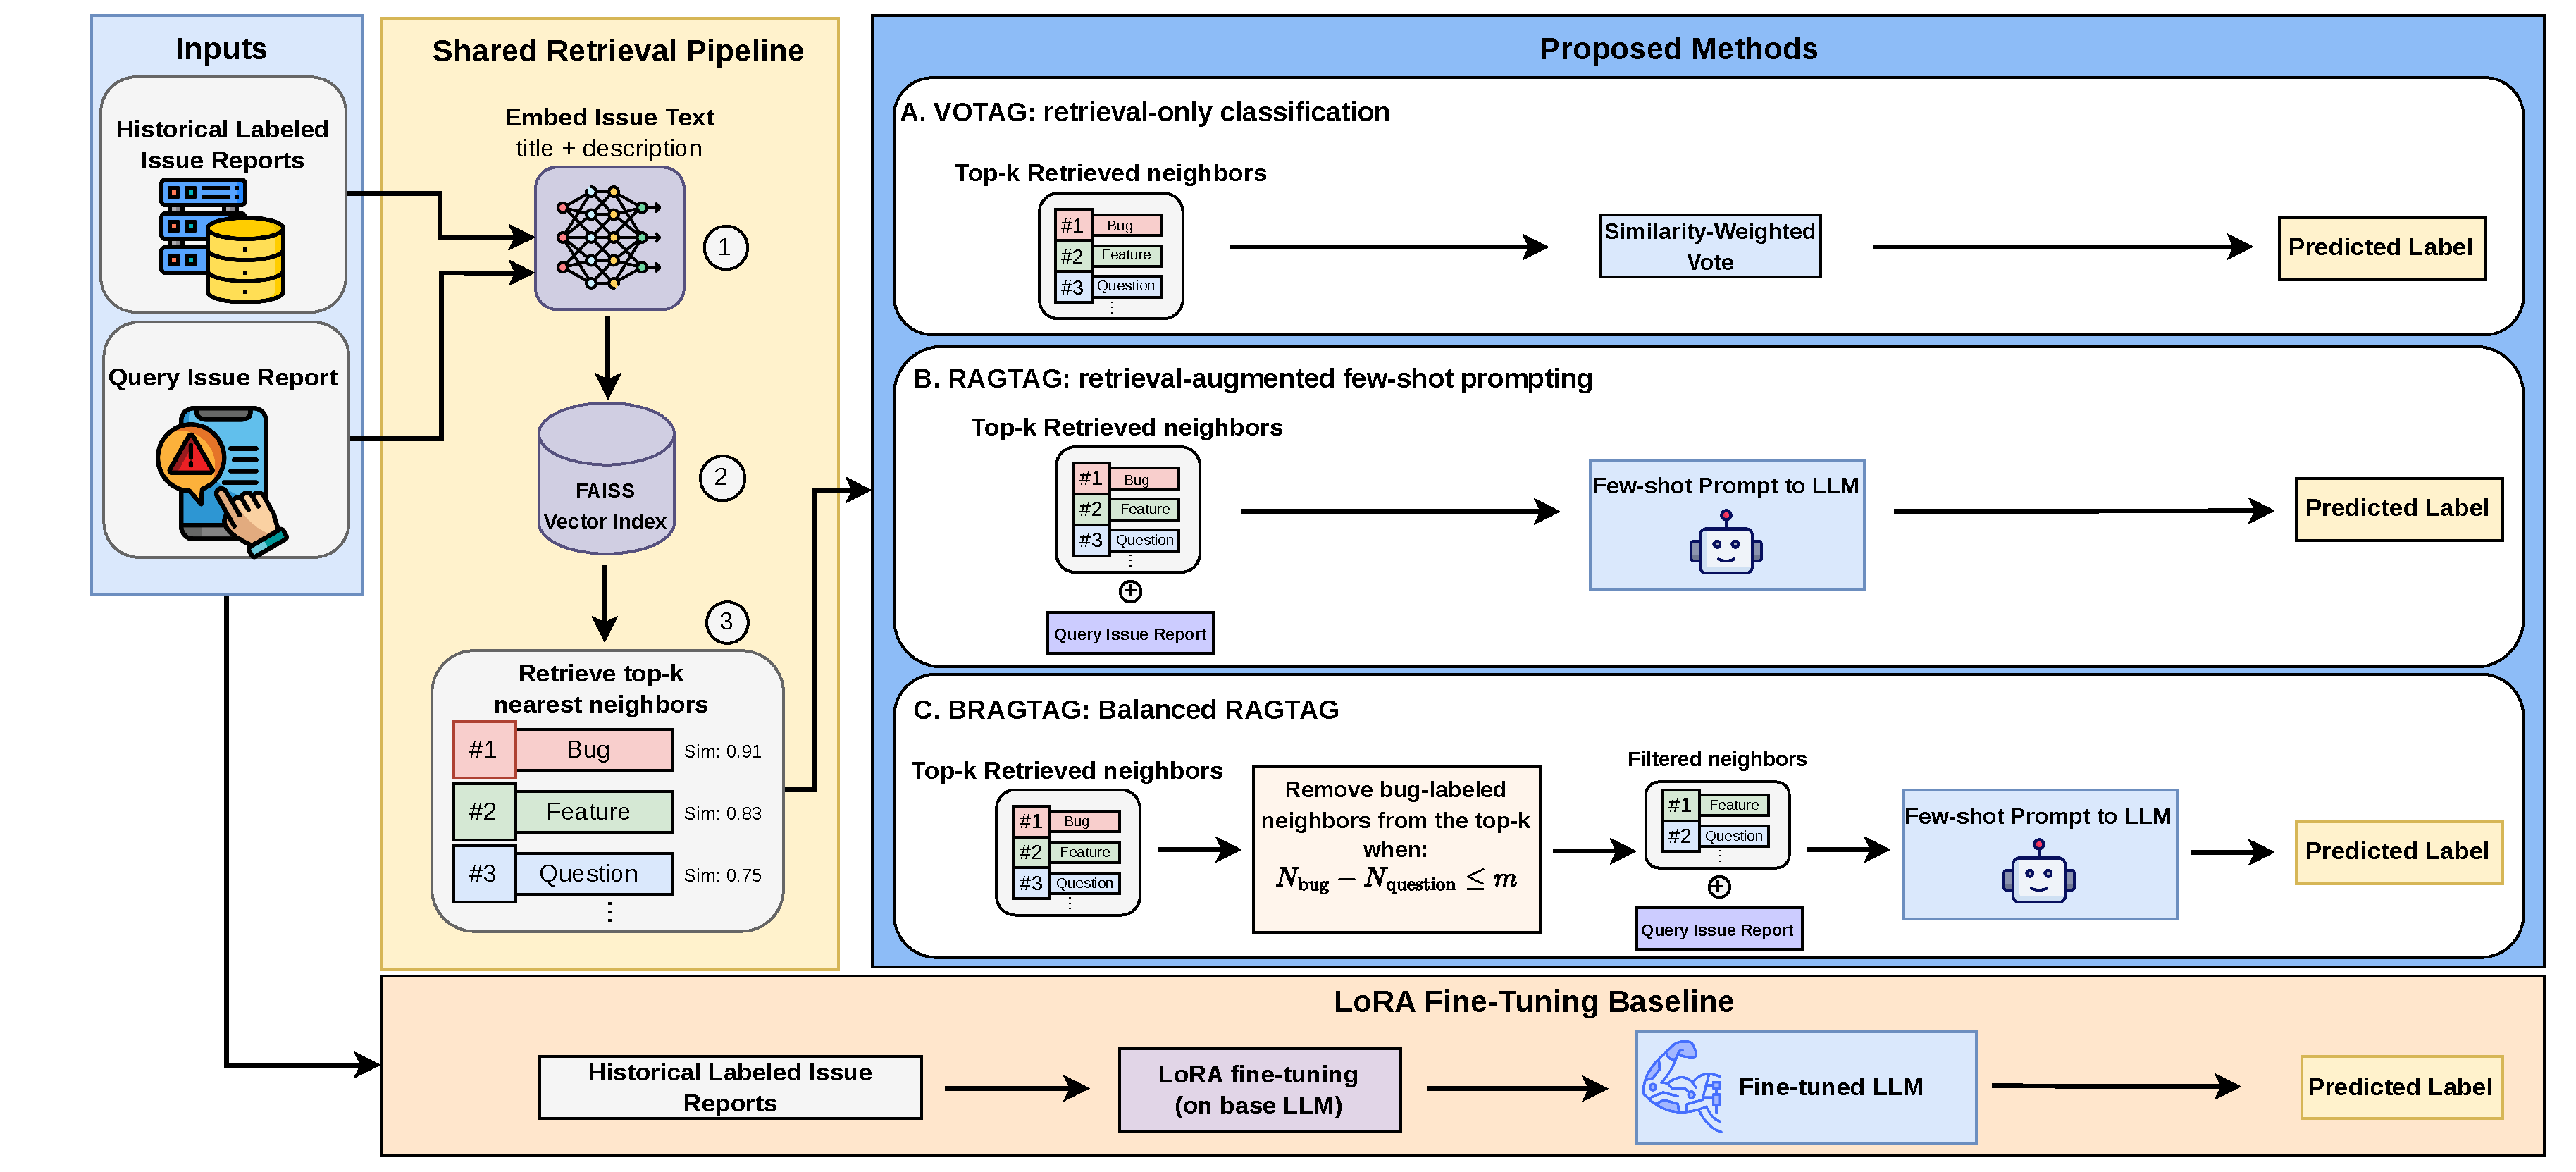
\includegraphics[width=0.88\textwidth]{figures/fao.pdf}
    \caption{Overview of the $k$NN voting baseline, retrieval-augmented few-shot prompting (RAG), filtered RAG, and the LoRA fine-tuning baseline.}
    \label{fig:approach-overview}
\end{figure*}

All retrieval-based classifiers share one retrieval step (\cref{sec:retrieval}). The \knn\ baseline labels the query from its neighbors' labels alone, \rag\ shows the neighbors to the LLM as labeled examples, and \frag\ removes bug-labeled examples for suspected questions. We compare the two RAG variants with LoRA fine-tuning of the same LLMs (\cref{sec:finetune}); \cref{fig:approach-overview} shows all four approaches.

\subsection{Problem Formulation}
\label{sec:problem}
Given a query issue report, we classify it into only one of the three labels: \emph{bug}, \emph{feature}, or \emph{question}. Only the issue's title and description text are used for classification with no other signals from the issue tracker. The defined label space is adopted directly from prior IRC studies~\cite{aracena2024applyinglargelanguagemodels,aracena2025applying,izadi2022catiss,kallis2019ticket,antoniol2008bug}. 

\subsection{Indexing and Retrieval}
\label{sec:retrieval}
To prepare the issues for retrieval based on textual similarity, we first embed their textual content (i.e., \textit{title} + \textit{description}). We do not embed the issue labels. Instead, we retain them as metadata associated with each embedded issue. To generate the embeddings, we use the \texttt{all-MiniLM-L6-v2} model from the Sentence-Transformers library~\cite{reimers2019sentence}. We selected this model due to its lightweight architecture, fast performance, and effectiveness on issue report text~\cite{huang2025back}. The embeddings are then indexed using the FAISS vector database library~\cite{douze2025faiss}, which provides efficient high-dimensional similarity retrieval. At the retrieval stage, the query issue is first embedded with the same model. Next, FAISS calculates the cosine similarity of indexed issue reports to the query, and returns the top-$k$ nearest neighbors, ordered by descending similarity.

%%%%%%%%%%%%%%%%%%%%
\subsection{$k$NN Voting Baseline}
\label{sec:approach-votag}
The \knn baseline labels the query by a similarity-weighted vote over the labels of its top-$k$ neighbors, following the distance-weighted $k$-nearest-neighbor rule~\cite{cover1967nearest, dudani1976distance}.\footnote{Squared-similarity weighting and uniform majority were also evaluated, but were outperformed by similarity-weighted voting.} Because it uses no LLM, \knn\ measures how much label information the neighbors carry. Its peak sets the largest $k$ we give the LLM (\cref{sec:rq1}), and it labels invalid LLM outputs in the fallback (\cref{sec:rq3}). Formally, for a
query issue $q$ with retrieved neighbors $\{(n_i, l_i, s_i)\}_{i=1}^{k}$, where
$n_i$ is the $i$-th nearest neighbor with label $l_i$ and cosine similarity $s_i$ to $q$, the predicted label $\hat{y}$ is given by:

\begin{equation}
    \hat{y} = \operatorname*{arg\,max}_{c \in \mathcal{L}}
    \sum_{i=1}^{k} s_i \cdot \mathbf{1}[l_i = c],
    \label{eq:votag}
\end{equation}

where $\mathcal{L}$ is the label set, and $\mathbf{1}[l_i = c]$ is the indicator function that equals $1$ when neighbor $i$ has label $c$ and $0$ otherwise. For each label, \knn\ sums the cosine similarities of the neighbors that carry that label, and the $\operatorname*{arg\,max}$ operator returns the label with the largest total sum. It breaks ties by returning the label of the most similar neighbor in the tied classes.



%%%%%%%%%%%%%%%%%%%%%%%%%%%%%%%%
\begin{comment} %% Prompt box with title bar
\definecolor{prompttitlebar}{HTML}{3A3A55}
\definecolor{promptbody}{HTML}{F2F2FF}
\begin{figure}[t]
    \centering
    \begin{tikzpicture}[
        font=\fontsize{6}{7}\selectfont\ttfamily,
        sec/.style={anchor=north, text width=10.3cm, align=left,
                    inner xsep=0.2cm, inner ysep=6pt, fill=promptbody},
        seclabel/.style={anchor=east, font=\sffamily\scriptsize,
                    align=right, text=prompttitlebar},
    ]
    % --- title bar ---
    \node[anchor=north, text width=10.3cm, align=center,
          inner xsep=0.2cm, inner ysep=4pt, fill=prompttitlebar,
          text=white, font=\sffamily\small\bfseries] (title) at (0,0)
        {Retrieval-augmented few-shot prompt format};
    % --- (1) system message ---
    \node[sec, below=0pt of title.south] (s1)
        {Classify the GitHub issue into exactly one category: bug, feature,
         or question. Respond with ONLY the label wrapped in XML tags
         (e.g., <label>bug</label>). Do NOT write anything else --- no
         explanation, no reasoning, no extra text.};
    % --- (2) retrieved examples ---
    \node[sec, below=0pt of s1.south] (s2)
        {Here are some examples of correctly classified issues:\\[2pt]
         -{}-{}- Example 1 -{}-{}-\quad Title: \textit{$\langle$title$\rangle$}\quad
         Body: \textit{$\langle$body$\rangle$}\quad
         Answer: <label>feature</label>\\[2pt]
         \textit{$\cdots$}\\[2pt]
         -{}-{}- Example K -{}-{}-\quad Title: \textit{$\langle$title$\rangle$}\quad
         Body: \textit{$\langle$body$\rangle$}\quad
         Answer: <label>bug</label>};
    % --- (3) query issue ---
    \node[sec, below=0pt of s2.south] (s3)
        {Now, classify the following target issue:\quad
         Title: \textit{$\langle$query title$\rangle$}\quad
         Body: \textit{$\langle$query description$\rangle$}};
    % --- dashed section dividers, extended beyond the border ---
    \draw[dashed] ([xshift=-1.9cm]s1.south west) -- ([xshift=0.35cm]s1.south east);
    \draw[dashed] ([xshift=-1.9cm]s2.south west) -- ([xshift=0.35cm]s2.south east);
    % --- outer border ---
    \draw[line width=0.8pt] (title.north west) rectangle (s3.south east);
    % --- section names, outside the border on the left ---
    \node[seclabel] at ([xshift=-0.22cm]s1.west) {System message};
    \node[seclabel] at ([xshift=-0.22cm]s2.west) {Retrieved examples\\($K$ nearest neighbors)};
    \node[seclabel] at ([xshift=-0.22cm]s3.west) {Query issue};
    \end{tikzpicture}
    \caption{The retrieval-augmented few-shot prompt structure used for \rag and
    \frag.}
    \label{fig:prompt}
\end{figure}
\end{comment}
%%%%%%%%%%%%%%%%%%%%%%%%%%%%%%%%

\definecolor{prompttitlebar}{HTML}{3A3A55}
\definecolor{promptbody}{HTML}{F2F2FF}

% Column-width prompt figure. Geometry: a 1.85cm label gutter on the left and a
% 0.10cm divider overhang on the right, so the drawing is exactly \columnwidth.
\begin{figure}[t]
    \centering
    \begin{tikzpicture}[
        font=\fontsize{6}{7}\selectfont\ttfamily,
        sec/.style={anchor=north, align=left,
                    text width=\dimexpr\columnwidth-2.0cm-0.4cm\relax,
                    inner xsep=0.2cm, inner ysep=5pt, fill=promptbody},
        seclabel/.style={anchor=east, font=\sffamily\scriptsize,
                    align=right, text=prompttitlebar, text width=1.55cm,
                    inner sep=0pt},
    ]

    % --- (1) system message ---
    \node[sec] (s1) at (0,0)
        {Classify the GitHub issue into exactly one category: bug, feature,
         or question. Respond with ONLY the label wrapped in XML tags
         (e.g., <label>bug</label>). Do NOT write anything else --- no
         explanation, no reasoning, no extra text.};

    % --- (2) retrieved examples ---
    \node[sec, below=0pt of s1.south] (s2)
        {Here are some examples of correctly classified issues:\\[2pt]
         -{}-{}- Example 1 -{}-{}-\quad Title: \textit{$\langle$title$\rangle$}\quad
         Body: \textit{$\langle$body$\rangle$}\quad
         Answer: <label>feature</label>\\[2pt]
         \textit{$\cdots$}\\[2pt]
         -{}-{}- Example $k$ -{}-{}-\quad Title: \textit{$\langle$title$\rangle$}\quad
         Body: \textit{$\langle$body$\rangle$}\quad
         Answer: <label>bug</label>};

    % --- (3) query issue ---
    \node[sec, below=0pt of s2.south] (s3)
        {Now, classify the following target issue:\quad
         Title: \textit{$\langle$query title$\rangle$}\quad
         Body: \textit{$\langle$query description$\rangle$}};

    % --- dashed section dividers, extended into the label gutter ---
    \draw[dashed] ([xshift=-1.85cm]s1.south west) -- ([xshift=0.10cm]s1.south east);
    \draw[dashed] ([xshift=-1.85cm]s2.south west) -- ([xshift=0.10cm]s2.south east);

    % --- outer border ---
    \draw[line width=0.8pt] (s1.north west) rectangle (s3.south east);

    % --- section names, in the gutter on the left ---
    \node[seclabel] at ([xshift=-0.15cm]s1.west) {System\\message};
    \node[seclabel] at ([xshift=-0.15cm]s2.west) {Retrieved\\examples\\($k$ nearest\\neighbors)};
    \node[seclabel] at ([xshift=-0.15cm]s3.west) {Query\\issue};

    \end{tikzpicture}
    \caption{The retrieval-augmented few-shot prompt structure used for \rag\ and
    \frag.}
    \label{fig:prompt}
\end{figure}
%%%%%%%%%%%%%%%%%%%%%%%%%%%%%%%%

\subsection{Retrieval-Augmented Few-Shot Prompting (RAG)}
\label{sec:approach-ragtag}
\rag shows the query's top-$k$ neighbors (\cref{sec:retrieval}) to the LLM as labeled examples. We use the neighbors, rather than randomly chosen labeled issues, because similar examples can outperform random ones~\cite{liu2022makes, yu2023retrieval} and because the neighbors' labels alone reach 59.5\% macro $F_1$ (\cref{sec:rq1}).
We create the few-shot prompt in three parts as shown in \figref{prompt}. First, the system message frames the classification task and the label space. Second, the top-$k$ nearest neighbors are listed in retrieval order (descending similarity), each formatted as \textit{title + description + label}. Finally, the query issue closes the prompt, since LLMs use information at the end of a long context better than in its middle~\cite{liu2024lost}. With $k{=}0$, the prompt has no examples and \rag\ becomes zero-shot prompting, as in prior work~\cite{colavito2025benchmarking}.

We evaluate $k \in \{0, 1, 3, 6, 9, 12, 15\}$, up to \knn's peaks at $k{=}15$--16 (\cref{sec:rq1}). The maximum prompt sequence length is set to 8,192 tokens.\footnote{Maximum prompt sequence length is selected empirically. 8,192 tokens offered the best trade-off between macro $F_1$ and inference speed across our preliminary experiments.} Roughly 30\% of the context quota is reserved for the query issue and 70\% for the neighbors. If the neighbors exceed their overall quota, they are truncated proportionally based on their length (longer neighbors get more truncation). The query issue gets truncated if it exceeds its budget as well. Truncation happens on the right side of the
description text, preserving all titles and labels (if any).
The LLM is instructed to generate the predicted label wrapped in XML tags (e.g. \texttt{<label>bug</label>}). The labels of the presented examples also follow the same format. We use a regular expression to extract the predicted label. Outputs that contain none of the three labels are marked as \textit{invalid}. Finally, models are loaded with Unsloth\footnote{\url{https://unsloth.ai}} for memory efficiency, and the temperature is set at 0.1 for deterministic classifications.
%%%%%%%%%%%%%%%%%%%%%
\subsection{Filtered RAG}
\label{sec:approach-bragtag}
\rag's most frequent error is labeling questions as bugs (\cref{sec:rq1}), a known weakness of \irc\ methods~\cite{colavito2024impact, colavito2025benchmarking}. The models make this error even at zero-shot, so we hypothesize that bug-labeled examples retrieved for a question reinforce it. \Frag\ therefore removes the bug-labeled examples from the prompt when the neighbors suggest that the query is a question, that is, when $N_\text{bug} - N_\text{question} \le m$, where $N_\text{label}$ is the number of neighbors with that label among the top $k$ and $m$ is a small positive margin. For example, with $k{=}12$ and $m{=}3$, a query whose neighbors are six bugs, four questions, and two features has $N_\text{bug} - N_\text{question} = 2$, so the six bug examples are removed and the prompt shows the remaining six.

We calibrated $m$ before testing, on a validation split of the labeled issues. From each project's 300 labeled issues, 30 issues stratified by label serve as queries and the other 270 as the retrieval index, mirroring the project-specific setting (\cref{sec:setup-dataset}). On this split, true questions retrieve nearly balanced bug and question neighbors, with on average 1.36 more question than bug neighbors over $k\in[1,15]$. We swept $m\in\{1,\dots,5\}$, where 5 is the 95th percentile of $N_\text{bug} - N_\text{question}$ for true questions, and chose $m{=}3$ as the best trade-off between firing for questions and for bugs. Averaged over $k$, it fires for 89.1\% of true questions and 56.7\% of true bugs. Otherwise, \frag\ is identical to \rag.

\subsection{LoRA Fine-Tuning Baseline}
\label{sec:finetune}
Prior LLM-based \irc\ studies fine-tune open LLMs on labeled issue reports with LoRA~\cite{hu2022lora, heo2025study, aracena2025applying}. Each training example is an instruction prompt with the issue's title and description as input and its label as output. We adopt the prompt template of these studies~\cite{heo2025study,aracena2025applying} verbatim, so that our baseline reproduces their method. At inference, the fine-tuned model receives the query issue in the same format and completes the empty label field. A regular expression extracts the label, and outputs that contain none of the three labels are \textit{invalid}.

Training hyperparameters follow prior work~\cite{heo2025study,aracena2025applying}. The LoRA rank and alpha are set to 16, with a learning rate of $2 \times 10^{-4}$ and the paged AdamW 8-bit optimizer. Training runs for 3 epochs with a per-device batch size of 1 and gradient accumulation steps of 16. The maximum prompt sequence length is 2,048 tokens, which leaves 94.9\% of the test issues untruncated; longer issues are truncated from the right of their description.
Similar to \rag and \frag, the models are loaded with Unsloth and the temperature is set at 0.1.

% !TEX root = ../SANER2027-main-labeling.tex
\section{Experimental Setup}
\label{sec:setup}

\myparagraph{Dataset and Settings}
\label{sec:setup-dataset}
We use the dataset introduced in Heo et al.~\cite{heo2025study} for our experiments. The dataset has a total of 6,600 issue reports gathered from eleven active open-source projects:
\texttt{ansible}, \texttt{bitcoin},
\texttt{dart-lang}, \texttt{roslyn},
\texttt{react}, \texttt{flutter},
\texttt{kubernetes}, \texttt{TypeScript},
\texttt{vscode}, \texttt{opencv}, and
\texttt{tensorflow}. Each project has 600 issue reports
with an equal distribution across the labels
(\emph{bug}, \emph{feature}, and \emph{question}). To support their LLM fine-tuning method, Heo et al. divided the dataset into 50/50 train and test
splits, stratified by project and label. This results in 300 train
and 300 test issue reports per project. We also adopt Heo et al.'s project-specific (PS) and project-agnostic (PA) configurations to examine how data scope affects IRC performance. In the PS setting, each project's train and test data are used in isolation, resulting in eleven different train-test pairs. In the PA setting, the train splits of all projects are merged into a single training set of 3,300 issue reports. In both configurations, \rag and \knn only use the training splits as their retrieval index to ensure fair comparison with the fine-tuning baseline.

%%%%%%%%%%%%
\myparagraph{Models}
\label{sec:setup-models}
We use the Qwen2.5-Instruct model family~\cite{yang2024qwen25} in our evaluations with four different parameter sizes: 3B, 7B, 14B, and 32B. Qwen2.5 is an open-source LLM with strong performance on general-purpose benchmarks. Using the same model with different parameter sizes enables analysis of the effect of model scale in LLM-based IRC approaches.


%%%%%%%%%%%%
\myparagraph{Evaluation Metrics}
\label{sec:setup-metrics}
We report the macro-averaged $F_1$ over the three labels as the headline metric, since it weighs the three labels equally. A method's \emph{best} $k$ (its best configuration) is the one with the highest macro $F_1$ on the test set. We report scores in percent and differences between methods in percentage points (points). We also report macro-averaged and per-class precision and recall. All metrics are calculated over the total 3{,}300-issue test set. We also report the rate of invalid outputs (\textit{invalid rate}), which count as incorrect predictions. For significance, we report bootstrap 95\% confidence intervals (CIs) on the macro $F_1$ differences between methods.\footnote{We resample the 3{,}300 test issues 1{,}000 times and evaluate both methods on the same resample (paired bootstrap).}

%%%%%%%%%%%%
\myparagraph{Hardware Setup}
\label{sec:setup-hardware}
Fine-tuning of Qwen-14B and Qwen-32B and the Qwen-32B runs at $k{\ge}12$ used one NVIDIA L40 or L40S GPU (48~GB VRAM). All other experiments used one NVIDIA RTX 4090 GPU (24~GB VRAM).

% !TEX root = ../SANER2027-main-labeling.tex
% Author revisions: blue (\fixed). Coauthor revision, 2026-09-21: magenta (\coauthor).
% Issue-level resampling done (2026-09-24); configuration-selection audit still pending.

\section{Evaluation}
\label{sec:evaluations}

In this section, we present the results of our experiments and answer the four research questions posed in \Cref{sec:01_intro}, one per subsection.
\fixed{Throughout this section, a method's \emph{best} $k$ or configuration is the one with the highest macro $F_1$.}
\fixed{\Cref{fig:kcurves} reports macro $F_1$ across the $k$ grid for the three retrieval-based methods, and \Cref{tab:results} lists every method at its best configuration, including the per-class precision and recall that RQ1--RQ4 refer to.}

% Presentation pass (2026-09-22): the eight floats of the previous draft (five figures,
% three tables) are consolidated into four: the k-curve figure and the master table
% below (full width, placed at the top of the section), the per-project heatmap (RQ4,
% now column width) and the CI table (RQ4). An error-profile figure (bug/question P-R
% planes, figures/error_profile.pdf) was drafted and dropped as redundant with the table.
% The +VOTAG (fallback) macro F1 column was moved out of the master table; the CI
% table's +VOTAG rows report the fallback as differences (author decision, 2026-09-22).
% Generators: scripts/paper/fig_kcurves.py, tab_results_master.py,
% fig_per_project_diff.py, tab_method_comparison_ci.py; all read paper/tables/*.csv
% and run on any machine.
\begin{figure*}[!t]
    \centering
    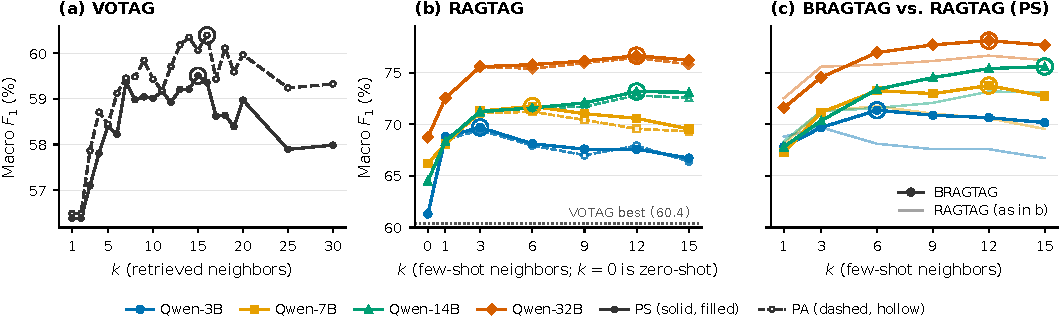
\includegraphics[width=\textwidth]{figures/kcurves.pdf}
    \caption{\fixed{Macro $F_1$ across the $k$ grid. \textbf{(a)}~\votag\ in PS (solid) and PA (dashed). \textbf{(b)}~\ragtag\ for the four Qwen sizes in PS (solid, filled) and PA (dashed, hollow). \textbf{(c)}~\bragtag\ (markers) against \ragtag. (b) and (c) share one $y$-axis and \fixed{rings} mark each method's best $k$.}}
    \label{fig:kcurves}
\end{figure*}
% Generated by scripts/paper/tab_results_master.py -- do not edit by hand.
\begin{table*}[!t]
  \centering
  \caption{Pooled test-set results of every method at its best configuration.}
  \label{tab:results}
  \footnotesize
  \renewcommand{\arraystretch}{0.97}
  \setlength{\tabcolsep}{6pt}
  \begin{tabular}{@{}llrrrrrrrrrrr@{}}
    \toprule
    Model & Method & $k$ & \multicolumn{2}{c}{Bug} & \multicolumn{2}{c}{Feature} & \multicolumn{2}{c}{Question} & $P_{\text{mac}}$ & $R_{\text{mac}}$ & Macro $F_1$ & Invalid \\
    \cmidrule(lr){4-5}\cmidrule(lr){6-7}\cmidrule(lr){8-9}
     & & & $P$ & $R$ & $P$ & $R$ & $P$ & $R$ & & & & (\%) \\
    \midrule
    -- & \votag\ (PS) & 15 & 0.552 & 0.734 & 0.677 & 0.562 & 0.592 & 0.498 & 0.607 & 0.598 & 0.595 & 0.0 \\
     & \votag\ (PA) & 16 & 0.556 & 0.731 & 0.689 & 0.579 & 0.600 & 0.508 & 0.615 & 0.606 & 0.604 & 0.0 \\
    \midrule
    Qwen-3B & Zero-shot & 0 & 0.543 & 0.915 & 0.886 & 0.610 & 0.568 & 0.353 & 0.666 & 0.626 & 0.613 & 0.2 \\
     & \ragtag\ (PS) & 3 & 0.638 & 0.803 & 0.794 & 0.813 & 0.694 & 0.494 & 0.709 & 0.703 & 0.697 & 0.2 \\
     & \bragtag\ (PS) & 6 & 0.723 & 0.665 & 0.794 & 0.813 & 0.644 & 0.646 & 0.720 & 0.708 & \textbf{0.714} & 1.8 \\
     & Fine-Tune (PS) & -- & 0.606 & 0.870 & 0.770 & 0.792 & 0.793 & 0.400 & 0.723 & 0.687 & 0.676 & 1.1 \\
     & Fine-Tune (PA) & -- & 0.637 & 0.873 & 0.833 & 0.751 & 0.724 & 0.511 & 0.731 & 0.712 & 0.708 & 0.8 \\
    \midrule
    Qwen-7B & Zero-shot & 0 & 0.575 & 0.881 & 0.792 & 0.789 & 0.783 & 0.367 & 0.717 & 0.679 & 0.662 & 0.1 \\
     & \ragtag\ (PS) & 6 & 0.657 & 0.824 & 0.787 & 0.848 & 0.838 & 0.474 & 0.761 & 0.715 & 0.718 & 3.5 \\
     & \bragtag\ (PS) & 12 & 0.713 & 0.774 & 0.761 & 0.855 & 0.825 & 0.558 & 0.766 & 0.729 & 0.738 & 3.8 \\
     & Fine-Tune (PS) & -- & 0.653 & 0.635 & 0.759 & 0.769 & 0.619 & 0.627 & 0.677 & 0.677 & 0.677 & 0.1 \\
     & Fine-Tune (PA) & -- & 0.672 & 0.878 & 0.868 & 0.825 & 0.800 & 0.588 & 0.780 & 0.764 & \textbf{0.762} & 0.3 \\
    \midrule
    Qwen-14B & Zero-shot & 0 & 0.570 & 0.876 & 0.761 & 0.855 & 0.873 & 0.294 & 0.735 & 0.675 & 0.645 & 0.1 \\
     & \ragtag\ (PS) & 12 & 0.651 & 0.844 & 0.839 & 0.836 & 0.855 & 0.489 & 0.782 & 0.723 & 0.732 & 4.5 \\
     & \bragtag\ (PS) & 15 & 0.696 & 0.803 & 0.836 & 0.844 & 0.832 & 0.579 & 0.788 & 0.742 & 0.756 & 4.7 \\
     & Fine-Tune (PS) & -- & 0.700 & 0.740 & 0.828 & 0.692 & 0.609 & 0.669 & 0.712 & 0.700 & 0.704 & 0.3 \\
     & Fine-Tune (PA) & -- & 0.730 & 0.865 & 0.882 & 0.781 & 0.764 & 0.710 & 0.792 & 0.785 & \textbf{0.785} & 0.0 \\
    \midrule
    Qwen-32B & Zero-shot & 0 & 0.611 & 0.861 & 0.766 & 0.869 & 0.857 & 0.387 & 0.745 & 0.706 & 0.688 & 0.2 \\
     & \ragtag\ (PS) & 12 & 0.701 & 0.828 & 0.855 & 0.828 & 0.840 & 0.598 & 0.799 & 0.752 & 0.767 & 4.6 \\
     & \bragtag\ (PS) & 12 & 0.748 & 0.804 & 0.847 & 0.833 & 0.808 & 0.664 & 0.801 & 0.767 & \textbf{0.781} & 4.0 \\
     & Fine-Tune (PS) & -- & 0.744 & 0.700 & 0.814 & 0.825 & 0.665 & 0.694 & 0.741 & 0.740 & 0.740 & 0.1 \\
     & Fine-Tune (PA) & -- & 0.689 & 0.929 & 0.832 & 0.876 & 0.895 & 0.534 & 0.805 & 0.780 & 0.771 & 0.1 \\
    \bottomrule
  \end{tabular}
  \par\vspace{2pt}
  \parbox{\textwidth}{\scriptsize PS: 300 labeled issues of the target project; PA: the 3{,}300 issues of all eleven projects. $P$/$R$: precision/recall; $P_{\text{mac}}$/$R_{\text{mac}}$: their macro averages. Invalid outputs count as incorrect. Bold: best macro $F_1$ per model size.}
\end{table*}


\subsection{RQ1: Effectiveness of Retrieval-Only IRC}
\label{sec:rq1}

\coauthor{We evaluate \votag\ in PS and PA at $k\in\{1,\ldots,20,25,30\}$ (\Cref{fig:kcurves}a). Similarity-weighted voting achieves its highest observed macro $F_1$ of 59.5\% at $k{=}15$ in PS and 60.4\% at $k{=}16$ in PA. Beyond these peaks, macro $F_1$ declines up to $k{=}30$. PA has slightly higher scores at every evaluated $k$. The small performance difference is consistent with the substantial overlap between retrieved neighbors: PS and PA share 84--90\% of their top-$k$ neighbors for the evaluated values between 3 and 30. Thus, even when the retrieval index includes all 3{,}300 training issues, most retrieved neighbors belong to the query's project.}

\coauthor{Question has the lowest class-specific $F_1$ at every evaluated $k$ in both settings. At the peak configurations, 32\% of question issues are predicted as bugs in both settings, compared with 18\% predicted as features in PS and 17\% in PA. Bug recall exceeds precision at every evaluated $k$, indicating that \votag\ over-predicts this class. At the peak configurations, bug recall is about 73\% and precision is 55--56\% (\Cref{tab:results}).}

\begin{coauthoranswer}
\coauthor{Retrieval-only voting achieves peak macro $F_1$ scores of 59.5\% with project-specific data and 60.4\% with pooled data. The small difference accompanies substantial overlap between retrieved neighbors. Question is the weakest class and is most often misclassified as bug.}
\end{coauthoranswer}

\subsection{RQ2: Effectiveness of Retrieval-Augmented Few-Shot IRC}
\label{sec:ragtag}

\coauthor{We evaluate \ragtag\ at $k\in\{0,1,3,6,9,12,15\}$ in PS and PA, where $k{=}0$ is the zero-shot baseline~\cite{colavito2025benchmarking}. \votag's peaks at $k{=}15$--16 (RQ1) set the upper end of this grid. \Cref{fig:kcurves}b reports macro $F_1$ across the grid in both settings.}

\coauthor{PS has slightly higher macro $F_1$ than PA at almost every (model, $k$) \fixed{pair} with $k{\ge}1$, using 300 in-project examples rather than a pool of 3{,}300. This small gap is consistent with the neighbor overlap in RQ1. Zero-shot predictions use no retrieval and are identical between settings. Below, \ragtag\ uses PS.}

\coauthor{All 48 nonzero-$k$ configurations, spanning four model sizes and both data scopes, outperform the corresponding zero-shot baseline and the strongest \votag\ configuration in macro $F_1$, macro precision, and macro recall. Thus, LLM classification using retrieved examples outperforms similarity-weighted voting. Within the PS grid, the \fixed{best $k$ is 3, 6, 12, and 12} for Qwen-3B, -7B, -14B, and -32B, respectively. These configurations achieve 69.7--76.7\% macro $F_1$, 7.6 points above zero-shot on average. Increasing $k$ from 12 to 15 does not improve any model's PS score.}

\coauthor{Question remains the weakest class by $F_1$ at every evaluated $k$ in both settings. It has the lowest recall but never the lowest precision. At zero-shot, 46--59\% of true-question issues are predicted as bugs, compared with 5--16\% predicted as features. These question-to-bug errors account for roughly 80\% of false bug predictions, linking the question-recall deficit to low bug precision.}

\coauthor{Retrieved examples reduce this confusion. At the best PS configurations, 26--36\% of question issues are predicted as bugs and 9--15\% as features. Averaged across the four models, the share of issues predicted as bug falls from 51\% to 42\%, bug precision increases from 57\% to 66\%, and question recall from 35\% to 51\% relative to zero-shot (\Cref{tab:results}). The increase in question-class $F_1$ accounts for 56--70\% of the macro-$F_1$ improvement across model sizes.}

\coauthor{The zero-shot results show that question-to-bug confusion exists before any examples are presented. We hypothesize that bug-labeled examples retrieved for true-question queries reinforce this tendency.} Based on this intuition, we propose a more balanced retrieval technique as an intervention that removes the bug-labeled neighbors whenever the query is a suspected question. We base the suspicion signal on the nearest neighbors' label distribution and calibrate it without including the test set. From each project's total 300 training issues, we assign 30 issues stratified by label as queries and 270 as the retrieval index, mirroring the PS setting. On this validation split, true-question queries retrieve almost balanced bug and question examples: averaged across $k\in[1,15]$, the mean of $N_\text{bug} - N_\text{question}$ is $-1.36$. We therefore treat a query as a suspected question when $N_\text{bug} - N_\text{question} \le m$, where $N_\text{label}$ is the count of neighbors with that label in the top-$k$ and $m$ is a small positive margin. Sweeping $m\in\{1,2,3,4,5\}$\footnote{We cap the sweep at $m{=}5$, since it is the 95th percentile of $N_\text{bug} - N_\text{question}$ on true-question queries.} on the validation split and averaging across $k\in[1,15]$, $m{=}3$ had a more favorable trade-off against the other values, firing for 89.1\% of true-question and 56.7\% of true-bug queries. We adopt $m{=}3$ and refer to the resulting method as \textbf{B}alanced \ragtag\ (\bragtag).

\begin{coauthoranswer}
\coauthor{Retrieved examples improve macro $F_1$, macro precision, and macro recall over zero-shot prompting and retrieval-only voting in every evaluated configuration with $k{\ge}1$. The best PS configurations achieve 69.7--76.7\% macro $F_1$. Question recall remains the principal weakness: 26--36\% of question issues are still classified as bugs, motivating the balanced retrieval intervention evaluated in RQ3.}
\end{coauthoranswer}

\subsection{RQ3: Effectiveness \fixed{and Trade-offs} of the Balanced Retrieval Method}
\label{sec:bragtag}

\coauthor{We compare \bragtag\ with \ragtag\ under PS at the same $k\in\{1,3,6,9,12,15\}$. At every tested $k\ge6$, \bragtag\ has higher macro $F_1$ for all four model sizes (\Cref{fig:kcurves}c)\fixed{, by at least 1.2 points}. At $k{=}1$ and $k{=}3$, its scores are lower by up to 1.0 point. With the fixed margin $m{=}3$, the condition $N_{\mathrm{bug}}-N_{\mathrm{question}}\le3$ holds for every query at these two small $k$ values. Bug-example removal is therefore unconditional, leaving no demonstrations for 40\% of queries at $k{=}1$ and 18\% at $k{=}3$.}

\coauthor{Comparing each method's best configuration, \bragtag\ increases macro $F_1$ by 1.5--2.4 points (\Cref{tab:results}).} \fixed{The 95\% CIs of these gains exclude zero for all four models, with lower bounds of 0.2--1.4 points}\footnote{1{,}000 paired bootstrap resamples per model.}. \fixed{\bragtag's} \coauthor{selected $k$ increases for the three smaller models and remains 12 for Qwen-32B.} When the trigger fires, \bragtag\ removes all bug examples from the top-$k$, so a higher initial $k$ is needed to leave enough context for the LLM.

\coauthor{The class-level results expose the trade-off. Question $F_1$ increases by 3.0--6.8 points, as recall rises by 6.5--15.3 points while precision falls by 1.2--5.0. Bug precision increases by 4.5--8.6 points, but bug recall decreases by 2.5--13.8 at every model size. The largest recall loss occurs for Qwen-3B, from 80.3\% to 66.5\%\fixed{, the one model where the intervention over-corrects}; its bug $F_1$ falls from 71.1\% to 69.3\%. Bug $F_1$ improves for the three larger models. Feature $F_1$ changes by \fixed{at most} 1.2 points. The full precision and recall values appear in \Cref{tab:results}.}

\coauthor{At these configurations, question-to-bug error rates decrease from 26--36\% with \ragtag\ to 19--27\% with \bragtag. Question-to-feature error rates change by at most 1.4 percentage points.} Averaged across $k\in[1,15]$, the question-to-bug rate drops from 31--40\% to 24--36\%. \fixed{The improvement is therefore a targeted reduction of question-to-bug confusion, at the cost of bug recall.} \coauthor{Invalid outputs remain counted as incorrect; their rates at these same configurations are reported in \Cref{tab:results} and analyzed in RQ4.}

\begin{myboxi}
\fixed{\bragtag\ outperforms \ragtag\ at every $k{\ge}6$ for all four model sizes. The gain is a targeted reduction of question-to-bug misclassifications: question $F_1$ rises by 3.0--6.8 points and bug precision by 4.5--8.6, at the cost of bug recall. Bug $F_1$ improves for the three larger models and drops by 1.8 points for Qwen-3B; feature $F_1$ changes by at most 1.2 points.}
\end{myboxi}

%\subsection{RQ4. Can retrieval-augmented few-shot prompting match LoRA fine-tuning for IRC, and what are the costs of each approach?}
\subsection{RQ4: Few-Shot Prompting vs. LoRA Fine-Tuning for IRC}
\label{sec:method-comparison}

% RQ4 rewrite (2026-09-19): five-step argument (same data -> best-vs-best ->
% error profile -> recall/invalid outputs -> fallback). TOST removed
% by author decision; paired bootstrap CIs only. All new text is blue (\fixed).
%
% Coauthor pass (2026-09-21, magenta \coauthor) reviewed 2026-09-22:
%   kept     invalid-output paragraph, fallback-protocol paragraph, fallback
%            results paragraph, CI table (now single-column), ext-table caption
%            detail on the fallback k values.
%   merged   PS/PA paragraph (0.060 rounding, PA confound, panel (b) sentence),
%            annotation-budget caveat, class-share caveat.
%   reverted section title, error-profile paragraph (author blue version),
%            "best observed" -> "best" (defined once in the S5 opener).
%   removed  encoder baselines (SetFit/RoBERTa) pending a separate decision;
%            tables/encoder_baselines.tex stays on disk but is not input.
%   cost     restored to the author's one-sentence version from c91bc26; the
%            coauthor's cost table and time discussion are dropped (not input).

%%%%%%%%%%%
\myparagraph{Classification Performance}

\fixed{We fine-tune all four models under both data scopes and compare them with \ragtag\ and \bragtag\ at their best $k$ (\Cref{tab:results}). When all methods use the same 300 labeled issues per project (PS), both retrieval-based approaches outperform fine-tuning at every model size: \ragtag\ leads by 2.1--4.0 points of macro $F_1$, and \bragtag\ by 3.8--6.0 points. Fine-tuning benefits from pooling the 3{,}300 labeled issues across all eleven projects (PA), which changes both the number of training examples and their project composition. Pooling raises its macro $F_1$ by 3.1--8.4 points relative to PS, consistent with prior findings~\cite{heo2025study}, although the class-level effects vary: for Qwen-32B, it increases bug recall but lowers question recall (\Cref{tab:results}).}

\fixed{The larger pool does not provide a corresponding benefit for retrieval (\Cref{sec:ragtag}). We therefore use PS for \ragtag\ and \bragtag\ and PA for fine-tuning in the remaining comparisons, giving each method its better-performing data scope. The eleven PS indexes collectively hold the same 3{,}300 training issues as the PA training set, so the two scopes differ in the data available per target project, not in the total annotation budget.}

% Generated by scripts/paper/tab_method_comparison_ci.py from paper/tables/method_comparison_ci.csv
% -- do not edit by hand. See the CSV header for the provenance of the current numbers.
\begin{table}[!t]
  \centering
  \caption{Macro-$F_1$ difference from PA fine-tuning in percentage points, without and with the \votag\ fallback (paired bootstrap 95\% CI).}
  \label{tab:method-comparison-ci}
  \footnotesize
  \setlength{\tabcolsep}{3pt}
  \begin{tabular}{@{}lrlrl@{}}
    \toprule
     & \multicolumn{2}{c}{\ragtag\ $-$ Fine-Tune} & \multicolumn{2}{c}{\bragtag\ $-$ Fine-Tune} \\
    \cmidrule(lr){2-3}\cmidrule(lr){4-5}
    Model & $\Delta F_1$ & 95\% CI & $\Delta F_1$ & 95\% CI \\
    \midrule
    Qwen-3B & $-1.1$ & $[-2.8, +0.7]$ & $+0.5$ & $[-1.2, +2.4]$ \\
    \quad +\votag & $-1.5$ & $[-3.2, +0.2]$ & $+0.9$ & $[-0.8, +2.8]$ \\
    \addlinespace[1.5pt]
    Qwen-7B & $\mathbf{-4.4}$ & $[-5.9, -2.9]$ & $\mathbf{-2.4}$ & $[-3.9, -0.9]$ \\
    \quad +\votag & $\mathbf{-3.3}$ & $[-4.7, -1.7]$ & $-1.1$ & $[-2.6, +0.4]$ \\
    \addlinespace[1.5pt]
    Qwen-14B & $\mathbf{-5.4}$ & $[-6.8, -3.9]$ & $\mathbf{-2.9}$ & $[-4.4, -1.3]$ \\
    \quad +\votag & $\mathbf{-4.0}$ & $[-5.4, -2.5]$ & $-1.4$ & $[-3.0, +0.1]$ \\
    \addlinespace[1.5pt]
    Qwen-32B & $-0.5$ & $[-2.0, +0.9]$ & $+1.0$ & $[-0.5, +2.4]$ \\
    \quad +\votag & $+0.8$ & $[-0.8, +2.2]$ & $\mathbf{+2.1}$ & $[+0.6, +3.5]$ \\
    \midrule
    All sizes & $\mathbf{-2.8}$ & $[-3.9, -1.8]$ & $-1.0$ & $[-2.0, +0.1]$ \\
    \quad +\votag & $\mathbf{-2.0}$ & $[-3.0, -1.0]$ & $+0.1$ & $[-0.9, +1.1]$ \\
    \bottomrule
  \end{tabular}
  \par\vspace{2pt}
  \parbox{\columnwidth}{\scriptsize \ragtag/\bragtag\ under PS at their best $k$, fine-tuning under PA; negative values favor fine-tuning. Each +\votag\ row applies the \votag\ fallback for invalid outputs to both methods. Bold: CI excludes zero. All sizes: mean of the four per-model differences.}
\end{table}


\fixed{\Cref{tab:method-comparison-ci} reports macro $F_1$ differences as the retrieval-based method minus fine-tuning, with paired bootstrap 95\% CIs.\footnote{We use 1{,}000 paired bootstrap resamples per comparison.} Averaged over the four model sizes, \ragtag\ trails fine-tuning by 2.8 points, and \bragtag\ trails it by 1.0 point, a gap whose CI includes zero. \ragtag\ trails fine-tuning at every model size, whereas \bragtag\ improves on \ragtag's difference at every size, to between 2.9 points behind and 1.0 point ahead. Fine-tuning is significantly ahead at Qwen-7B and Qwen-14B. At Qwen-3B and Qwen-32B, the confidence intervals include zero, and \bragtag\ has the higher point estimates. Results also vary by project: \bragtag\ matches or exceeds PA fine-tuning in 16 of the 44 (project, model) pairs, including all four sizes on \texttt{opencv} and three of four on \texttt{bitcoin} (\Cref{fig:per-project-diff}).}

\begin{figure}[!t]
    \centering
    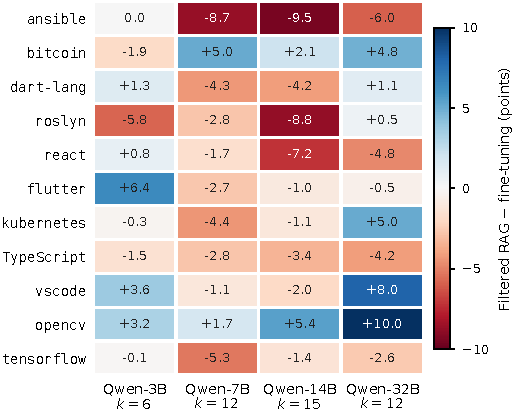
\includegraphics[width=\columnwidth]{figures/per_project_diff.pdf}
    \caption{\fixed{Macro $F_1$ difference in percentage points between \bragtag\ (PS, best $k$) and PA LoRA fine-tuning on each project's 300 test issues, for the four model sizes. Blue favors \bragtag, red favors fine-tuning.}}
    \label{fig:per-project-diff}
\end{figure}

\fixed{Fine-tuning detects more actual bugs at every model size, while \bragtag\ makes fewer false bug predictions at three of the four sizes. Like the zero-shot models (\Cref{sec:ragtag}), the PA fine-tuned models over-predict bug: they assign this label to 39--46\% of test issues, although only 33\% are bugs. Their bug recall is high (86--93\%), but precision is lower (64--73\%), and 23--36\% of question issues are classified as bugs. \bragtag\ predicts bug for 31--38\% of issues, closer to the true share, and misclassifies 19--27\% of questions as bugs. Its bug recall is lower (66--80\%), while its precision is generally higher (70--75\%). The one size at which \bragtag\ does not make fewer false bug predictions is Qwen-14B, where fine-tuning's tendency to over-predict bug is less pronounced: it labels 39.5\% of issues as bugs and misclassifies 23\% of questions as bugs. A bug share close to the true proportion is not by itself evidence of quality; what matters is the trade-off between bug recall and bug precision, and which method is preferable depends on the relative cost of missed bugs and incorrect bug assignments in a given project.}

\coauthor{At Qwen-7B and Qwen-14B, \bragtag's macro recall is lower than LoRA's by 3.5 and 4.3 points, respectively, while its macro precision is within 1.5 points of LoRA's at every size. Invalid outputs contribute to this recall deficit: they count as false negatives for the true class without adding a prediction to any valid class's precision denominator. At the selected configurations, invalid rates are 0.2--4.6\% for \ragtag, 1.8--4.7\% for \bragtag, and at most 0.8\% for LoRA. For \bragtag\ at Qwen-7B and larger sizes, 6--8\% of true bugs receive invalid outputs.}

\coauthor{We therefore compare complete pipelines that assign a valid label to every issue by applying a \votag\ fallback only when the LLM output is invalid. The fallback uses PS voting at fixed $k{=}15$ for \ragtag/\bragtag\ and PA voting at fixed $k{=}16$ for LoRA. It uses the original, unfiltered neighbors, independently of the number of demonstrations shown to the LLM. The retrieval-based pipelines can reuse their cached neighbor pool; adding this fallback to LoRA introduces a retrieval step. No additional LLM calls are required.}

\coauthor{After applying the fallback to all three LLM approaches (\Cref{tab:method-comparison-ci}, +\votag\ rows), \bragtag\ ranges from 1.4 points behind LoRA to 2.1 points ahead. Its deficits at Qwen-7B and Qwen-14B are approximately halved, to 1.1 and 1.4 points, while its Qwen-32B lead grows to 2.1 points. LoRA's scores change by at most 0.3 points.} \fixed{On average, \bragtag\ is then 0.1 points ahead of fine-tuning, with a CI that includes zero, and per model the interval excludes zero only at Qwen-32B, in \bragtag's favor.}

%%%%%%%%%%%%%%%%%%%%%
\myparagraph{Computation and Data Cost}

% \begin{figure}[t]
%     \centering
%     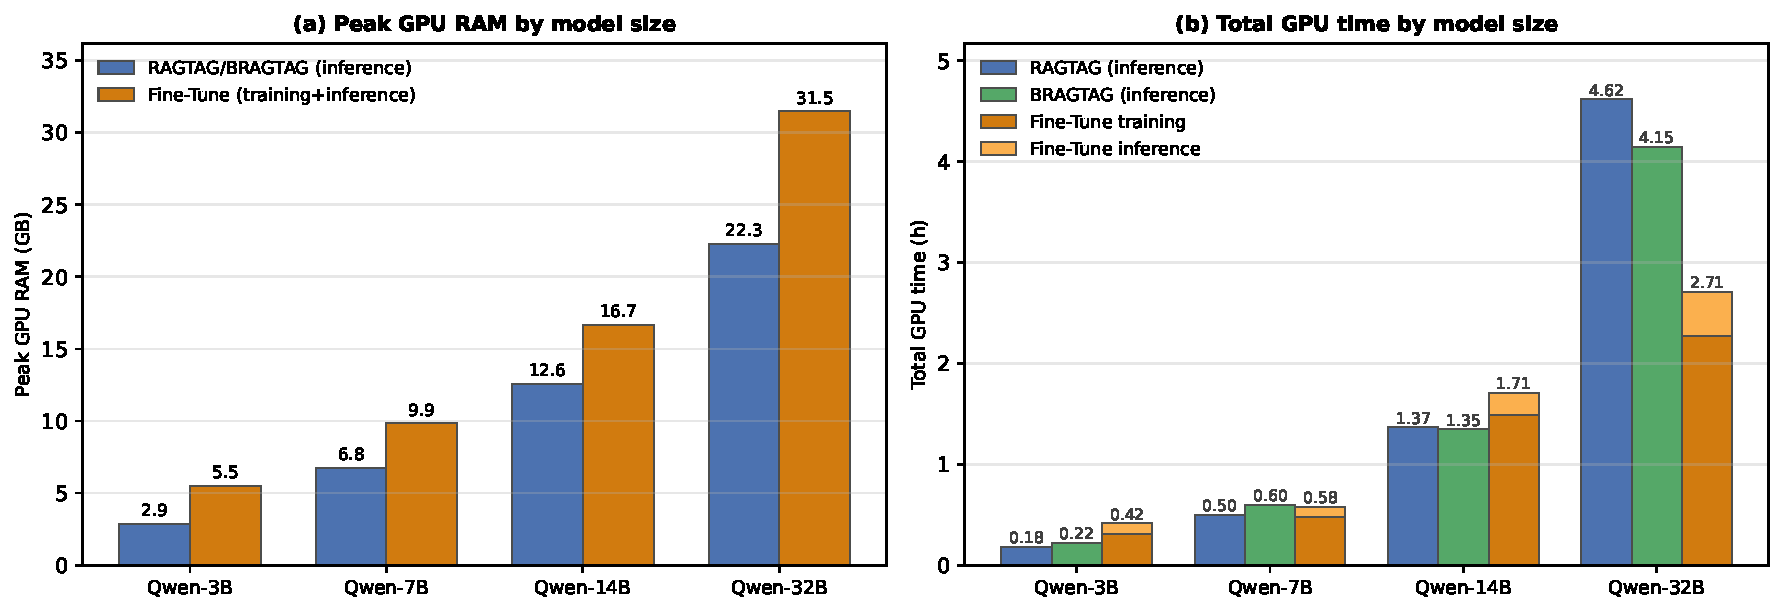
\includegraphics[width=\linewidth]{figures/cost_analysis.pdf}
% \caption{\textbf{(a)} Peak GPU memory by model size for \ragtag/\bragtag\ inference compared with LoRA fine-tuning training plus inference. \textbf{(b)} Total GPU time by model size for \ragtag\ and \bragtag\ compared with LoRA fine-tuning.}
%     \label{fig:cost-analysis}
% \end{figure}

% Author's shortened version (commit c91bc26), restored 2026-09-22; "per project"
% added to match the annotation-budget caveat earlier in this subsection.
% tables/method_cost.tex input again 2026-09-24, with the time trade-off below.
% Savings from peak GPU memory in GB, RAG vs. LoRA incl. training: 2.9/5.5, 6.8/9.9, 12.6/16.7, 22.3/31.5.
% VOTAG cost measured 2026-09-24 (tables/method_cost.tex header).
\begin{table}[t]
  \centering\color{blue}
  \caption{Computational cost of \ragtag, \bragtag, and LoRA fine-tuning at the configurations of \Cref{tab:method-comparison-ext}. RAM is the observed peak GPU memory; Train and Infer are wall-clock runtimes on a single GPU (\ragtag/\bragtag\ have no training phase), and Total is their sum, excluding model load.}
  \label{tab:method-cost}
  \footnotesize
  \setlength{\tabcolsep}{3.5pt}
  \begin{tabular}{llcccc}
    \toprule
    Model & Method & RAM (GB) & Train (h) & Infer (h) & Total (h) \\
    \midrule
    Qwen-3B & \ragtag & 2.9 & -- & 0.18 & 0.18 \\
     & \bragtag & 2.9 & -- & 0.22 & 0.22 \\
     & Fine-Tune & 5.5 & 0.31 & 0.11 & 0.42 \\
    \addlinespace[2pt]
    Qwen-7B & \ragtag & 6.8 & -- & 0.50 & 0.50 \\
     & \bragtag & 6.8 & -- & 0.60 & 0.60 \\
     & Fine-Tune & 9.9 & 0.48 & 0.10 & 0.58 \\
    \addlinespace[2pt]
    Qwen-14B & \ragtag & 12.6 & -- & 1.37 & 1.37 \\
     & \bragtag & 12.6 & -- & 1.35 & 1.35 \\
     & Fine-Tune & 16.7 & 1.49 & 0.22 & 1.71 \\
    \addlinespace[2pt]
    Qwen-32B & \ragtag & 22.3 & -- & 4.62 & 4.62 \\
     & \bragtag & 22.3 & -- & 4.15 & 4.15 \\
     & Fine-Tune & 31.5 & 2.28 & 0.44 & 2.71 \\
    \bottomrule
  \end{tabular}
\end{table}


\fixed{Our RAG-based methods require 47\%, 31\%, 25\%, and 29\% less peak GPU memory than LoRA fine-tuning for Qwen-3B, -7B, -14B, and -32B, respectively (33\% on average), while using $11\times$ less labeled data per project (\Cref{tab:method-cost}). They have no training phase, but their inference takes longer. Fine-tuned models label the 3{,}300 test issues in 0.10--0.44~h, whereas \ragtag\ and \bragtag\ take 0.18--4.62~h. Including training, \bragtag\ takes less total time than fine-tuning at Qwen-3B and Qwen-14B, about the same at Qwen-7B, and more at Qwen-32B (4.15~h versus 2.71~h). Without an LLM, \votag\ labels the 3{,}300 test issues in under 4~s with 0.2~GB of GPU memory, at a macro $F_1$ of 59.5\% (\Cref{sec:rq1}).}

\begin{myboxi}
% \textbf{Answer to RQ4:} 
\fixed{Averaged over the four model sizes, \bragtag\ with only the target project's labeled issues achieves a macro $F_1$ statistically indistinguishable from that of fine-tuning on all eleven projects' labeled issues, while needing no training, $11\times$ less labeled data per project, and 33\% less peak GPU memory. Per model size, the difference is significant only at Qwen-7B and Qwen-14B, in fine-tuning's favor, and, with a \votag\ fallback for invalid outputs, only at Qwen-32B, in \bragtag's favor. Without balancing, \ragtag\ trails fine-tuning by 2.8 points on average. When fine-tuning also uses only the target project's labeled issues, \ragtag\ and \bragtag\ score higher than it at every model size. Fine-tuning detects more bugs but over-predicts the bug class, whereas \bragtag\ makes fewer false bug predictions.}
\end{myboxi}

% !TEX root = ../SANER2027-main-labeling.tex
% Discussion: failure analysis and implications.

\section{Discussion}
\label{sec:discussion}

\subsection{Failure Analysis}
\label{sec:disc-failures}

We manually analyzed the errors of Qwen-32B at each method's best configuration. We randomly sampled 50 misclassified issues each from \rag, \frag, and LoRA fine-tuning, 150 in total. Each method's sample has 30 true-question, 10 true-bug, and 10 true-feature errors, which mirrors the label distribution of the errors pooled over the three methods. Two authors analyzed each case independently and resolved disagreements through discussion. We found three categories.

\myparagraph{Wrong template (116 of 150, 77\%)} The issue's content and label contradict the template it was filed under. All of these errors are questions and feature requests filed under a bug-report template (\textit{Steps to reproduce}, \textit{Expected}, \textit{Actual}, \textit{System Information}), whose structure leads the LLM to predict bug regardless of the content. For example, \texttt{vscode\#193985}\footnote{\url{https://github.com/microsoft/vscode/issues/193985}} is a support question that opens with a literal \texttt{Type:Bug} because it uses VS Code's bug template.

\myparagraph{Hybrid intent (20 of 150, 13\%)} The issue combines intents and could defensibly carry more than one label, mostly because a fix or a feature request is layered into a question or bug report. For example, in \texttt{kubernetes\#120364}\footnote{\url{https://github.com/kubernetes/kubernetes/issues/120364}} the author reports a concrete bug and, in the same body, requests a new feature: ``\textit{Please, give us multiarchitecture image! and fix monoarchitecture images too!}''

\myparagraph{Label noise (14 of 150, 9\%)} The ground-truth label does not match the content. For example, \texttt{tensorflow\#61710}\footnote{\url{https://github.com/tensorflow/tensorflow/issues/61710}}, titled ``\textit{Will there be an MLP model in the future version?}'', requests a new API feature but is labeled as a bug.

Wrong templates affect all three approaches. We hypothesize that the headings of a bug template are a strong cue for the bug label, both for the retriever, which then returns bug-labeled neighbors, and for the LLM itself. The other two categories are harder for any text-based classifier. For the 34 errors with hybrid intent or label noise (23\%), another label is defensible or the ground truth is wrong, so they limit the macro $F_1$ that any classifier can reach on this benchmark.

We also sampled 30 invalid outputs each from \rag\ and \frag. In 44 of the 60 cases (73\%), the model continued the issue body or its own reasoning. In 14 (23\%), it produced degenerate text such as repeated digits and punctuation. In the remaining 2 (3\%), it gave a label outside the three, such as \texttt{documentation}.

\subsection{Implications}
\label{sec:disc-implications}

\myparagraph{Labeled data and retraining} With \frag, a project's own labeled issues give, without training and with 33\% less peak GPU memory, a macro $F_1$ within 1.0 point of fine-tuning on $11\times$ as many issues pooled from eleven projects; the difference is not statistically significant, while \rag\ trails by 2.8 points (\Cref{sec:rq3}). The comparison is starker for a project that cannot draw on other projects' labeled issues: fine-tuned on the same issues, the model scores 3.8--6.0 points below \frag. Building the index for a project needs only its labeled issues and one embedding pass, whereas pooled fine-tuning needs labeled issues collected from other projects. A new labeled issue then becomes an index update rather than a retraining run, so the examples can follow a project as its issues change, and the LLM can be replaced by a newer one without retraining.

\myparagraph{Where fine-tuning keeps an edge} Fine-tuning keeps three advantages. It is significantly ahead at Qwen-7B and Qwen-14B, the sizes at which pooling the eleven projects' issues helps it most (\Cref{sec:rq3}). Its inference is faster, most clearly at Qwen-32B, where \frag\ takes longer in total even when fine-tuning's training is included; this advantage grows with the number of issues labeled between two training runs. And it almost never produces invalid outputs, whereas the RAG variants need the \knn\ fallback to give every issue a valid label.

\myparagraph{Error profiles} The approaches differ less in macro $F_1$ than in which errors they make. Fine-tuning finds more bugs at every size, whereas \frag\ raises fewer false bug alarms at three of the four sizes. Macro $F_1$ weighs both errors equally, but their costs need not be equal: a false bug label costs a triager's time, whereas a missed bug can delay a fix. Neither approach removes the question-to-bug confusion.

\myparagraph{Question-to-bug confusion} The confusion persists under every method we test, including fine-tuning, as in prior \irc\ work (\Cref{sec:02_related}). The filter reduces it without training but cannot remove it. Many of the remaining errors are questions filed under a bug template (\Cref{sec:disc-failures}), which read like bug reports to the retriever and the LLM alike.

\myparagraph{Retrieval alone as a floor} Without an LLM, \knn\ reaches 59.5\% macro $F_1$, 1.8 points below Qwen-3B's zero-shot prompting, with 0.2 instead of 2.9~GB of GPU memory. Neither the neighbors' labels nor the LLM alone reaches the scores of \rag, which outperforms both at every size (\Cref{sec:rq1}); the gain comes from giving the LLM the labeled neighbors.

\myparagraph{Classification and templates} Our failure analysis shows that users often file support questions and feature requests under the bug-report template, which leads the classifier to predict bug regardless of the content. Most of the sampled errors are of this kind, so correcting the template when an issue is filed could prevent many of them. This matters for the LLM-assisted triage now offered on platforms such as GitHub~\cite{githubcopilot} and GitLab~\cite{gitlabduo}, where the reporter describes the issue to an LLM that suggests a template and labels. Report validation matters as well, since mislabeled and duplicate reports are common~\cite{antoniol2008bug, pandey2017automated}. Prior studies validate bug reports~\cite{khatib2025assertflip, wang2024aegis, ahmed2025otter, dincc2025judge}, but combining classification and validation in one workflow remains underexplored.

% !TEX root = ../SANER2027-main-labeling.tex
% Threats to Validity

\section{Threats to Validity}
\label{sec:threats}

\myparagraph{Internal Validity} Each method's best $k$ is the one with the highest macro $F_1$ on the test set, which favors the RAG variants. With a single $k{=}12$ for every model size, \frag\ trails fine-tuning by 1.2 points on average instead of 1.0 (\Cref{sec:rq3}). The filter's margin was calibrated on a validation split of the labeled issues, not on the test set, and is the same for all models and projects (\Cref{sec:approach-bragtag}). Prompts and hyperparameters affect fine-tuning results~\cite{heo2025study,aracena2025applying}. Ours follow prior work where it reports them (\Cref{sec:finetune}), and other choices could change the results of either approach. Invalid outputs count as errors, which penalizes the RAG variants most; the fallback analysis shows their effect (\Cref{sec:rq3}). The issues are public and may appear in the LLMs' pretraining data, which would affect zero-shot prompting and both approaches, since all use the same models.

\myparagraph{Construct Validity} Macro $F_1$ on a balanced three-label test set weighs the labels equally, and we report per-class precision and recall so that trade-offs between labels stay visible (\Cref{tab:results}). Some ground-truth labels are wrong, accounting for 9\% of the sampled errors (\Cref{sec:disc-failures}). Since all methods are scored against the same labels, this noise lowers every method's scores. LLM outputs can vary between runs, so we ran the experiments three times and report the average. The failure analysis covers 150 sampled errors of Qwen-32B, so its shares are estimates and may differ at other sizes. Times depend on the GPU, and at Qwen-14B, fine-tuning and the RAG variants ran on different GPUs (\Cref{sec:setup-hardware}).

\myparagraph{Conclusion Validity} We test differences between methods with paired bootstrap CIs that resample the test issues (\Cref{sec:setup-metrics}). The per-size comparisons are not corrected for multiple comparisons, so a single per-size result should be read with care; the headline rests on the average over the four sizes. The CIs resample issues, not projects, so they do not capture the variation across projects, which reaches about 10 points on single projects (\Cref{fig:per-project-diff}).

\myparagraph{External Validity} We study one model family (Qwen2.5-Instruct, four sizes), one embedding model, and one benchmark of eleven GitHub projects with balanced labels. Results may differ with imbalanced labels, other issue trackers, or other model families. The $11\times$ ratio follows from pooling eleven projects with 300 labeled issues each, and other numbers of projects or of labeled issues per project may change the gap between the approaches. Issue text also varies in writing style, vocabulary, and structure across projects~\cite{akhavan2026linkanchorautonomousllmbasedagent}, and our results vary by project as well (\Cref{fig:per-project-diff}).

% !TEX root = ../SANER2027-main-labeling.tex
% Conclusion
% Claims to support: summary + future work

\section{Conclusion and Future Work}
\label{sec:conclusion}

\begin{comment}
We evaluate all three against a LoRA fine-tuning baseline on an 11-project benchmark, in both \emph{project-specific} (PS) and \emph{project-agnostic} (PA) data scope settings. Experiments use Qwen2.5-Instruct at four sizes.
In this study, we investigated retrieval-augmented few-shot prompting as a cost-efficient alternative to LoRA fine-tuning for issue report classification (IRC). Given a query issue, we retrieved its top-$k$ nearest neighbors from historical issue reports to be used in three proposed methods. First, \rag, which presents the neighbors as labeled examples in a few-shot prompt. Second, \frag, a \rag\ variant that drops bug-labeled neighbors when the retrieved label distribution indicates the query is likely a question. Third, \knn, which predicts the label by a weighted vote on the neighbors' labels, establishing a non-parametric baseline. 

We evaluated all three methods against the LoRA fine-tuning baseline using the Qwen2.5-Instruct model at four sizes. Evaluations were conducted under both project-specific (PS) and project-agnostic (PA) data scope settings.
The results show that retrieval-augmented few-shot prompting is a practical alternative to fine-tuning for IRC. \rag\ PS outperforms fine-tuning PS by 0.021--0.040 macro $F_1$ across all four model sizes, and trails fine-tuning PA by 0.029 macro $F_1$ in aggregate despite using 11$\times$ less labeled data per project. \frag\ PS closes this gap to TOST equivalence at $\delta{=}0.02$, tightening to statistical equivalence at $\delta{=}0.01$ under the \knn\ fallback protocol for invalid LLM outputs. Averaged across all models, retrieval-augmented few-shot also required 33\% less peak GPU memory than fine-tuning.

These findings position retrieval-augmented few-shot prompting as the more practical IRC method, particularly when hardware is constrained, labeled data is limited, or deployment requires frequent model or data updates. We encourage future work to evaluate these methods in diverse data distribution scenarios and to explore additional retrieval techniques and configurations.

%%%%%%% Future Work
Future work should examine the generalizability of our findings beyond the studied benchmark by evaluating IRC methods under more diverse conditions, including imbalanced label distributions, minority-class scenarios, multi-label classification, and other issue tracking platforms such as Jira and Bugzilla. Additional work should also explore stronger retrieval-side interventions, such as LLM-based filtering or re-ranking of retrieved neighbors, as well as the effects of different embedding models and similarity metrics on retrieval quality. Finally, future studies should investigate alternative prompt structures, including advanced strategies such as Chain-of-Thought prompting~\cite{koyuncu2025exploring}, and evaluate other open-source LLM families to better understand how model architecture influences retrieval-augmented few-shot IRC.
\end{comment}

In this study, we investigated retrieval-augmented few-shot prompting (\rag) as a training-free alternative to LoRA fine-tuning for issue report classification (\irc). We conducted an empirical study with four Qwen2.5-Instruct models and 6{,}600 issue reports from eleven projects, where the retrieval index and the fine-tuning data come either from the target project's 300 labeled issues or from all 3{,}300 labeled issues of the eleven projects. We first tested how well the labels of a query issue's most similar neighbors predict its label, using a similarity-weighted vote over them (\knn). Since these neighbors carry label information, \rag gives them to the LLM as few-shot examples. Because \rag\ most often labels questions as bugs, a filtered variant (\frag) removes the bug-labeled examples for suspected questions.

Retrieved examples improve the LLM over both zero-shot prompting and \knn, and \frag\ improves on \rag\ by reducing question-to-bug errors, at the cost of bug recall. With the same labeled issues of the target project, \rag\ and \frag\ at their best number of examples outperform LoRA fine-tuning at every model size. When fine-tuning instead uses all 3{,}300 labeled issues of the eleven projects, it outperforms \rag, while its lead over \frag\ is not statistically significant. With \knn\ replacing invalid LLM outputs, \frag\ matches fine-tuning (+0.001 macro~$F_1$ on average). Fine-tuning finds more of the actual bugs but over-predicts the bug label, whereas \frag\ makes fewer false bug predictions at most model sizes, and the question-to-bug confusion persists under every method we test. Needing only the target project's labeled issues and 33\% less peak GPU memory on average, retrieval-augmented few-shot prompting is a competitive, training-free alternative to LoRA fine-tuning.

The two approaches trade different strengths, and which one suits a project depends on its labeled data, its GPU budget, and whether a missed bug or a false bug label costs it more. With retrieval, a newly labeled issue only needs to be indexed, and the LLM can be replaced without retraining. As this work constitutes a case study on the Qwen2.5-Instruct family, future work can focus on the generalizability of these findings by extending them to other LLM families and quantization settings to further strengthen or bound the conclusions drawn here. Additional directions include examining imbalanced label distributions, minority-class scenarios, multi-label classification, and other issue tracking platforms such as Jira and Bugzilla. Further research should also explore stronger retrieval-side interventions, such as LLM-based filtering or re-ranking of retrieved neighbors, as well as the effects of different embedding models and similarity metrics on retrieval quality. Finally, future studies should investigate alternative prompt structures, including advanced strategies such as Chain-of-Thought prompting~\cite{koyuncu2025exploring}.

% !TEX root = ../SANER2027-main-labeling.tex
% Data Availability
% SANER 2027 requires a Data Availability statement immediately after the
% Conclusion (unnumbered section, before References).

\section*{Data Availability}
\label{sec:data_availability}
Our replication package~\cite{replication_package} contains the code, data, and all necessary materials to reproduce the results presented in this paper.
   % mandatory, directly after Conclusion

%%%%%%%%%%%%%%%%%%%%%%%%%%%%%%%%%%%%%%%%%
%%          References
%%%%%%%%%%%%%%%%%%%%%%%%%%%%%%%%%%%%%%%%%
\balance
\bibliographystyle{IEEEtran}
\bibliography{refs}

\end{document}
